\subsection{Local reach certificates}
\label{subsec:reach-certificates}

For the nonzero-gap finite residuals, noncontainment by a unit C triangle is
certified through the exact local admissible set.  A backward boundary reach
and a radial reach bound the forward reach of the same V triangle; the next
edge then supplies the following backward reach.  These calculations are not
a separate global strategy.  They prove the inequalities used by
Proposition~\ref{prop:residual-hull-enclosure} in the five surviving
nonzero-gap families.  We retain the common equilateral-enclosure calculus,
the center-assisted path budget, the exceptional T3-like and Vd placements,
and the complete branchwise certificates.  Formalization-only optimization
registries remain repository interfaces and are not repeated in print.

\begingroup
\let\PrintedSubsection\subsection
\let\PrintedSubsubsection\subsubsection
\let\PrintedParagraph\paragraph
\let\section\PrintedSubsection
\renewcommand{\subsection}[1]{\PrintedSubsubsection{#1}\leavevmode\par}
\renewcommand{\subsubsection}[1]{\PrintedParagraph{#1}\leavevmode\par}
\section{Universal Enclosure and Transfer Calculus}
\label{sec:universal-calculus}

This section collects the geometry shared by the transfer and direct-witness
arguments.  The same equilateral enclosure functional governs the local
admissible set of Strategy~2 and the forced witness set of Strategy~4.  The
same radical governs the signed center, all selected $T_+$ arcs, and the
standard local frontiers.  Strategy~2 uses one decorated $g$-family: a hat
imposes the nonsupercritical cap, $\vee$ takes the complementary
incoming-reach view, and extra subscripts or superscripts record center
intervals or lower relaxations.

\subsection{The equilateral enclosure gauge}

Let $\mathsf R$ denote counterclockwise rotation through $2\pi/3$.  For a
nonempty compact set $K\subset\mathbb R^2$, put
\[
 h_K(n)=\max_{x\in K}\langle x,n\rangle
\]
and
\begin{equation}
 \Lambda(K)=\frac2{\sqrt3}
 \min_{\lVert n\rVert=1}
 \sum_{j=0}^2h_K(\mathsf R^jn).
 \label{eq:universal-lambda}
\end{equation}

\begin{proposition}[Equilateral enclosure gauge]
\label{prop:universal-enclosure-gauge}
The number $\Lambda(K)$ is the least side length of a closed equilateral
triangle containing $K$.  It is monotone under inclusion, translation
invariant, and positively homogeneous.  If $K$ is a finite polygonal hull, a
minimizing normal may be chosen perpendicular to one of its hull edges.
\end{proposition}

\begin{proof}
For a fixed unit normal $n$, the three supporting half-planes with outward
normals $n,\mathsf Rn,\mathsf R^2n$ form an equilateral triangle.  Its side is
$2/\sqrt3$ times the sum of the three support numbers, which proves
\eqref{eq:universal-lambda}.  Monotonicity and homogeneity are immediate, while
translation invariance follows from
\[
 n+\mathsf Rn+\mathsf R^2n=0.
\]
On an open normal-direction cell with three fixed support points, the support
sum has the form $A\cos\theta+B\sin\theta$ and has second derivative equal to
its negative.  In the nondegenerate case an interior critical point is a
maximum.  Hence a minimum occurs at a cell boundary, where one support line
contains a hull edge.
\end{proof}

For the local demand hull
\[
 K(a,b,c)=\conv\{0,au,bv,c(u+v)\},
\]
where $u$ and $v$ are the two unit boundary directions meeting at $120^\circ$,
the admissible set is
\begin{equation}
 \mathcal A
 =\{(a,b,c)\in[0,1]^3:\Lambda(K(a,b,c))\le1\}.
 \label{eq:universal-admissible-gauge}
\end{equation}
The exact support cells and radial envelope are proved in
Appendix~\ref{sec:exact-local-demand-calculus}.

\subsection{One equilateral radical}

For $0\le x\le1$, define
\begin{equation}
 \omega(x)=\sqrt{1-x+x^2},
 \qquad
 \sigma(x)=1-\omega(x).
 \label{eq:universal-radical}
\end{equation}
Then
\begin{equation}
 \omega(1-x)=\omega(x),
 \qquad
 \sigma(x)=\frac{x(1-x)}{1+\omega(x)},
 \label{eq:universal-radical-identities}
\end{equation}
and direct differentiation gives
\begin{equation}
 \sigma''(x)=-\frac3{4\omega(x)^3}<0.
 \label{eq:universal-sigma-concavity}
\end{equation}
Thus $\sigma$ is strictly concave.  In the signed center calculus,
\[
 E=\omega(R),\qquad \eta=\sigma(R).
\]

For $0<x<1$, put $z=\sigma(x)/x$.  Eliminating the square root gives
\begin{equation}
 x=\frac{1-2z}{1-z^2},
 \qquad
 \sigma(x)=\frac{z(1-2z)}{1-z^2},
 \qquad 0<z<\frac12.
 \label{eq:universal-rational-radical}
\end{equation}
This is the common rational parameter used in the selected high-sheet
calculations.

\subsection{One \(g\)-family}

For $0\le x,c\le1$, define the historical defect-coordinate map
\begin{equation}
 g_c(x)
 =
 \max\{y\in[0,1]:(1-x,y,c)\in\mathcal A\},
 \qquad
 \widehat g_c(x)=\min\{g_c(x),x\}.
 \label{eq:reader-raw-capped-maps}
\end{equation}
Thus $x$ is the incoming boundary defect, $g_c(x)$ is the exact maximal
outgoing reach, and the hat imposes the nonsupercritical diagonal cap.

For any map $f:[0,1]\to[0,1]$, put
\begin{equation}
 f^\vee(a)=1-f(1-a).
 \label{eq:reader-complement-dual}
\end{equation}
Hence
\begin{equation}
 \widehat g_c^\vee(a)
 =
 1-\widehat g_c(1-a)
 \ge a.
 \label{eq:reader-capped-raw-relation}
\end{equation}

The exact appendix aliases are
\begin{equation}
 B_c(a)=g_c(1-a),
 \qquad
 F_c(a)=\widehat g_c(1-a),
 \qquad
 G_c(a)=\widehat g_c^\vee(a).
 \label{eq:reader-technical-aliases}
\end{equation}
They are retained only where they shorten the contact-cell algebra.

\begin{lemma}[Raw and capped actual-row transfer]
\label{lem:reader-raw-capped-transfer}
Suppose an actual row has incoming reach at least $a$, radial reach at least
$c$, and outgoing reach $B$.  If no center interval intervenes on the next
edge, then
\[
 B\le g_c(1-a),
 \qquad
 A_{\rm next}\ge g_c^\vee(a).
\]
If the row is nonsupercritical, then
\[
 B\le\widehat g_c(1-a),
 \qquad
 A_{\rm next}\ge\widehat g_c^\vee(a)\ge a.
\]
\end{lemma}

\begin{proof}
The same triangle realizes $(a,B,c)$, so the definition of $g_c$ gives
$B\le g_c(1-a)$.  A center-free boundary handoff gives
\[
 A_{\rm next}\ge1-B\ge1-g_c(1-a)=g_c^\vee(a).
\]
Under nonsupercriticality one also has $B\le1-a$, so
$B\le\min\{g_c(1-a),1-a\}=\widehat g_c(1-a)$.  Taking complements proves the
last assertion.
\end{proof}

\begin{proposition}[Zero-radial distinction]
\label{prop:reader-zero-radial-g}
For $0<x<1$,
\[
 g_0(x)>x,
 \qquad
 \widehat g_0(x)=x,
\]
and therefore
\[
 g_0^\vee(a)<a,
 \qquad
 \widehat g_0^\vee(a)=a
 \quad(0<a<1).
\]
\end{proposition}

\begin{proof}
The exact diameter formula is
\[
 B_0(a)=\frac{-a+\sqrt{4-3a^2}}2.
\]
Consequently
\[
 g_0(x)=B_0(1-x)
 =\frac{x-1+\sqrt{1+6x-3x^2}}2.
\]
Since
\[
 1+6x-3x^2-(1+x)^2=4x(1-x)>0,
\]
one has $g_0(x)>x$.  The hatted identity follows from its definition, and the
dual statements follow by complementation.
\end{proof}

\subsection{Center-assisted transfers and the free envelope}

Let $J\subseteq[0,1]$ be empty or a closed interval.  For $0\le p\le1$, put
\[
 e_J(p)=\sup\{x\in[0,1]:[0,x]\subseteq[0,p]\cup J\},
 \qquad
 \mathcal R_J(p)=1-e_J(p).
\]
If $J=[L,U]$, then
\begin{equation}
 \mathcal R_{[L,U]}(p)=
 \begin{cases}
  1-p,&p<L,\\
  1-\max\{p,U\},&p\ge L,
 \end{cases}
 \qquad
 \mathcal R_\varnothing(p)=1-p.
 \label{eq:reader-residual-formula}
\end{equation}
The map is nonincreasing in $p$ and under enlargement of $J$.

\begin{lemma}[Generalized boundary handoff]
\label{lem:reader-generalized-handoff}
Suppose a unit boundary edge is covered by a left trace contained in $[0,p]$,
a center trace $J$, and a right trace contained in $[1-q,1]$.  Then
\[
 q\ge\mathcal R_J(p).
\]
For an actual row as in Lemma~\ref{lem:reader-raw-capped-transfer}, define
\[
 g_{c,J}^\vee(a)
 =
 \mathcal R_J(g_c(1-a)).
\]
Then
\begin{equation}
 A_{\rm next}
 \ge \mathcal R_J(B)
 \ge g_{c,J}^\vee(a).
 \label{eq:reader-generalized-raw-transfer}
\end{equation}
If the row is nonsupercritical, define
\[
 \widehat g_{c,J}^\vee(a)
 =
 \mathcal R_J(\widehat g_c(1-a)).
\]
Then
\begin{equation}
 A_{\rm next}
 \ge \widehat g_{c,J}^\vee(a).
 \label{eq:reader-generalized-transfer}
\end{equation}
For $J=\varnothing$, these are $g_c^\vee$ and
$\widehat g_c^\vee$.
\end{lemma}

\begin{proof}
The component of $[0,p]\cup J$ containing $0$ is $[0,e_J(p)]$.  If
$1-q>e_J(p)$, the intervening open interval is uncovered.  Hence
$q\ge1-e_J(p)$.  The remaining assertions follow from the outgoing bounds in
Lemma~\ref{lem:reader-raw-capped-transfer} and the fact that $\mathcal R_J$ is
nonincreasing.
\end{proof}

For $0\le c<1/2$, define the single free strict-supercritical envelope
\begin{equation}
 g_c^{\rm sc}
 =
 \sup_{\{x:g_c(x)>x\}}g_c(x)
 =
 \frac{c+\sqrt{c^2-8c+4}}2.
 \label{eq:reader-free-supercritical-envelope}
\end{equation}
The supremum is not attained.  Therefore an actual strict-supercritical row
with radial demand at least $c$ satisfies
\begin{equation}
 B<g_c^{\rm sc},
 \qquad
 A_{\rm next}>1-g_c^{\rm sc}.
 \label{eq:reader-free-raw-envelope}
\end{equation}
The former notation was
$B_{\rm sc}(c)=g_c^{\rm sc}$ and
$A_{\rm sc}(c)=1-g_c^{\rm sc}$.

\subsection{Relaxed composition and path budgets}

For maps listed in geometric row order, write
\begin{equation}
 [\Phi_1\mid\cdots\mid\Phi_r](x)
 =
 (\Phi_r\circ\cdots\circ\Phi_1)(x).
 \label{eq:reader-chain-notation}
\end{equation}
The leftmost slot acts first.  Write $\mathrm I(x)=x$ and $\mathrm I^k$ for
$k$ consecutive identity slots.

\begin{lemma}[Relaxed composition]
\label{lem:reader-relaxed-composition}
Suppose actual demands satisfy
\[
 x_j\ge\Phi_j(x_{j-1})
 \qquad(1\le j\le r),
\]
where every $\Phi_j$ is nondecreasing.  If
$\underline\Phi_j\le\Phi_j$, then
\[
 x_r\ge
 [\underline\Phi_1\mid\cdots\mid\underline\Phi_r](x_0).
\]
\end{lemma}

\begin{proof}
Set $y_0=x_0$ and
$y_j=\underline\Phi_j(y_{j-1})$.  If $x_{j-1}\ge y_{j-1}$, then
\[
 x_j
 \ge\Phi_j(x_{j-1})
 \ge\Phi_j(y_{j-1})
 \ge\underline\Phi_j(y_{j-1})
 =y_j.
\]
Induction proves the claim.
\end{proof}

\begin{lemma}[Boundary-path budget]
\label{lem:reader-boundary-path}
Let $T_1,\ldots,T_k$ be roles on a chain of $k+1$ consecutive unit boundary
edges.  If the two external endpoint roles contribute at most $u$ and $v$ on
the first and last edges, then coverage forces
\begin{equation}
 \sum_{j=1}^k(A_j+B_j)\ge k+1-u-v.
 \label{eq:reader-path-budget}
\end{equation}
Consequently, if all $k$ internal rows are nonsupercritical, the chain is
impossible whenever $u+v<1$.
\end{lemma}

\begin{proof}
The first and last edges give $A_1\ge1-u$ and $B_k\ge1-v$.  Each middle edge
gives $B_j+A_{j+1}\ge1$.  Adding these $k+1$ inequalities proves
\eqref{eq:reader-path-budget}.
\end{proof}

\subsection{Low-root and order-transition parameters}

For the high-radial maps used later, define
\begin{equation}
 e(d)=\frac{1-d}{2}
 \left(1-\sqrt{4(1-d)^2-3}\right)
 \qquad
 \left(0<d<1-\frac{\sqrt3}{2}\right).
 \label{eq:signed-low-root-definition}
\end{equation}
For the low-radial order transition, put
\begin{equation}
 h(c)=\frac{2c}{1+\sqrt{16c^2-3}}
 \qquad\left(\frac12<c\le\frac{\sqrt3}{2}\right).
 \label{eq:signed-order-transition}
\end{equation}
The exact contact-cell calculation in
Appendix~\ref{sec:exact-local-demand-calculus} proves that $e(d)$ is the low
selected root for radial demand $1-d$ and that $h(c)$ is the transition
between the two selected $T$ orders.

\subsection{The universal selected-\(T_+\) curve}

\begin{proposition}[Universal selected-$T_+$ curve]
\label{prop:reader-universal-tplus}
Fix $0<d<1/2$, put $c=1-d$, and suppose an input $p$ belongs to a selected
$T_+$ arc of $\widehat g_c^\vee$.  Write
\[
 q=\widehat g_c^\vee(p),
 \qquad \nu=q-p,
 \qquad x=\frac{q-d}{1-d}.
\]
Then
\begin{equation}
 \nu=\sigma(x)=1-\sqrt{1-x+x^2},
 \label{eq:reader-psi}
\end{equation}
and
\begin{equation}
 q=d+(1-d)x,
 \qquad
 p=d+(1-d)x-\sigma(x).
 \label{eq:reader-tplus-normal}
\end{equation}
Consequently $p\mapsto\widehat g_{1-d}^\vee(p)$ is increasing and strictly
concave on every selected $T_+$ arc.
\end{proposition}

\begin{proof}
The selected quadratic is
\[
 (1-q)(q-d)=(1-d)^2\nu(2-\nu).
\]
Substitution of $q=d+(1-d)x$ gives
\[
 x(1-x)=\nu(2-\nu).
\]
The selected component uses the smaller root, namely $\nu=\sigma(x)$.  For
fixed $d$, the function
\[
 p_d(x)=d+(1-d)x-\sigma(x)
\]
is increasing and strictly convex by \eqref{eq:universal-sigma-concavity}.
Its inverse is increasing and strictly concave, and $q=d+(1-d)x$ is affine in
that inverse.
\end{proof}

With the low root in \eqref{eq:signed-low-root-definition}, the high-radial chord
is
\begin{equation}
 \widehat g_{1-d}^\vee(p)
 \ge p+\frac{d}{e(d)-d}(p-d).
 \label{eq:reader-high-chord}
\end{equation}
If $t=h(1-d)$ is the low-radial order transition, the corresponding chord is
\begin{equation}
 \widehat g_{1-d}^\vee(p)
 \ge p+\frac{1-2t}{t-d}(p-d).
 \label{eq:reader-low-chord}
\end{equation}

To avoid a new function letter, for every coefficient $\lambda$ proved valid
on a selected arc write
\begin{equation}
 \widehat g_{1-d}^{\vee,\lambda}(p)
 :=
 p+\lambda(p-d)
 \le
 \widehat g_{1-d}^\vee(p).
 \label{eq:reader-affine-relaxation}
\end{equation}
The superscript $\lambda$ denotes a lower relaxation, not a second exact map.

The rational form \eqref{eq:universal-rational-radical} gives, in the
historical notation $x=1-\beta$,
\begin{equation}
 \beta=\frac{z(2-z)}{1-z^2},
 \qquad
 m_\beta=\frac{1-z+z^2}{1-z^2}.
 \label{eq:reader-beta-rational}
\end{equation}

\subsection{Threshold routing}

For $0<d<1-\sqrt3/2$, the exact high-demand threshold is
\begin{equation}
 z>e(d)
 \quad\Longrightarrow\quad
 \widehat g_{1-d}^\vee(z)\ge1-e(d).
 \label{eq:reader-high-threshold}
\end{equation}
Define the decorated lower threshold transfer
\begin{equation}
 \widehat g_{1-d}^{\vee,\rm th}(z)
 =
 \begin{cases}
  z,&z\le e(d),\\
  1-e(d),&z>e(d).
 \end{cases}
 \qquad
 \widehat g_{1-d}^{\vee,\rm th}
 \le
 \widehat g_{1-d}^\vee.
 \label{eq:reader-threshold-transfer}
\end{equation}

\begin{lemma}[Threshold routing]
\label{lem:reader-threshold-routing}
Let $z_j=\Phi_j(z_{j-1})$, where every $\Phi_j$ is nondecreasing and extensive.
If $\Phi_k=\widehat g_{1-d}^\vee$ and $z_{k-1}>e(d)$, then
\[
 z_j\ge1-e(d)\qquad(j\ge k).
\]
If a chain contains later occurrences of
$\widehat g_{1-d_1}^\vee$ and $\widehat g_{1-d_2}^\vee$ and
\[
 z_0>e(d_1),
 \qquad
 \min\{e(d_1),e(d_2)\}<Q,
\]
then one of those two rows forces every subsequent output above $1-Q$.
\end{lemma}

\begin{proof}
Equation~\eqref{eq:reader-high-threshold} gives the first triggered output,
and extensivity preserves it.  For the two-threshold statement, if
$e(d_1)<Q$, trigger at the first row.  Otherwise
\[
 z_0>e(d_1)\ge Q>e(d_2),
\]
so trigger at the second row.
\end{proof}

The lemma is used only after an actual-row induction such as
\eqref{eq:reader-generalized-raw-transfer} or
\eqref{eq:reader-generalized-transfer} has identified every formal iterate as
a lower bound for the corresponding actual row.

\endgroup

% The signed variables are defined in Section 2; execute their local reach
% interface here, after the canonical maps have been introduced.
\SignedCenterPropagation

\begingroup
\let\PrintedSubsection\subsection
\let\PrintedSubsubsection\subsubsection
\let\PrintedParagraph\paragraph
\let\section\PrintedSubsection
\renewcommand{\subsection}[1]{\PrintedSubsubsection{#1}\leavevmode\par}
\renewcommand{\subsubsection}[1]{\PrintedParagraph{#1}\leavevmode\par}
\section{Exceptional Local Profiles and Vd Placements}
\label{sec:short-vd-placements}

% STATEMENTS-ONLY-REPLACE-BEGIN: vd-profile-introduction
This subsection proves the local profile estimates used by the
one-special-triangle branches.  A T3-like adjacent exceptional triangle and a
Vd1 adjacent exceptional triangle satisfy the same two scalar
inequalities and therefore share one center-hiding theorem.  The remaining
Vd1/Vd2 placements use the interval residuals from
Section~\ref{sec:universal-calculus}, one global radial envelope, and two
immediate consequences of the corner normal form.
% STATEMENTS-ONLY-REPLACE-END: vd-profile-introduction

Use the strict-supercritical envelope $M_c^{\rm sup}$ from
\eqref{eq:reader-free-supercritical-envelope}; its explicit formula is
strictly decreasing for $0\le c<1/2$.  At $c=1/2$ we use only the continuous
extension $M_{1/2}^{\rm sup}=1/2$.  The strict feasible set is empty there,
so this endpoint value is never described as an attained supremum.

\subsection{A global quarter radial envelope}

For $(p,h)\in[0,1]^2$, let $c_{\max}(p,h)$ be the maximal radial coordinate
such that $(p,h,c)$ belongs to the local admissible set.

\begin{lemma}[Quarter radial envelope]
\label{lem:quarter-radial-envelope}
If
\[
 0\le h\le p,
 \qquad
 p+h<1,
\]
then
\begin{equation}
 c_{\max}(p,h)\le1-\frac h4.
 \label{eq:quarter-radial-envelope}
\end{equation}
The inequality is strict on the selected $\mathcal A_T$ component.
\end{lemma}

\begin{proof}
Put $s=p+h$ and $q=s^4-s^2+ph$.  Since $s<1$, only the two
nonsupercritical cells of Proposition~\ref{prop:exact-admissible-set} occur.

On $\mathcal A_L$, the smaller boundary coordinate is $h$, and the selected
radial frontier is the unique root in $[\sqrt3/2,1]$ of
\[
 P_h(c)=c^4-c^2+hc-h^2=0.
\]
At $c_0=1-h/4$,
\[
 P_h(c_0)=\frac h{256}(h^3-16h^2-240h+128).
\]
The cubic decreases on $[0,1/2]$ and has value $33/8$ at $1/2$, so this is
positive for $h>0$.  Moreover
\[
 P_h\left(\frac{\sqrt3}{2}\right)
 =-\left(h-\frac{\sqrt3}{4}\right)^2\le0,
 \qquad
 P_h'(c)>0\quad(c\ge\sqrt3/2).
\]
Hence the selected root is below $c_0$; for $h=0$ equality gives
$c_{\max}=1$.

On $\mathcal A_T$, put
\[
 r=\sqrt{4s^2-3},
 \qquad
 \gamma=\frac{p-h}{s}.
\]
The exact identity
\[
 \frac q{s^2}=\frac{r^2-\gamma^2}{4}
\]
gives $0\le\gamma<r$.  Write $\gamma=wr$, $0\le w<1$.  Then
\[
 p=\frac{s(1+wr)}2,
 \qquad
 h=\frac{s(1-wr)}2,
 \qquad
 c_{\max}=\frac{s(1+wr)}{1+r}.
\]
For
\[
 \Psi(w)=c_{\max}+\frac h4
\]
one has
\[
 \Psi'(w)=\frac{sr(7-r)}{8(1+r)}>0,
\]
so
\[
 \Psi(w)<\Psi(1)=\frac{s(9-r)}8.
\]
Since $4s^2=r^2+3$,
\[
 256-(r^2+3)(9-r)^2
 =(1-r)(r^3-17r^2+67r+13)>0
\]
for $0\le r<1$; the cubic is increasing and positive on this interval.
Thus $s(9-r)<8$ and $c_{\max}+h/4<1$.
\end{proof}

\subsection{The rational T3-like adjacent-exception profile}

\begin{lemma}[T3-like adjacent-exception profile]
\label{lem:short-t3-rescuer-profile}
Let a translated T3-like triangle at $V_0$ contain $M_1$, have boundary trace
$[0,a]$ on $e_{5,0}$, and have trace $[c,u]$ on $r_1$ measured
from $V_1$ toward $O$.  Then
\begin{equation}
 a\le 1-M_c^{\rm sup},
 \qquad
 \frac{a}{a+1-u}\le 1-M_c^{\rm sup}.
 \label{eq:short-t3-profile}
\end{equation}
\end{lemma}

\begin{proof}
The translated T3-like normal form supplies
\[
 1\le D\le\frac2{\sqrt3},
 \qquad
 E=\sqrt{4-3D^2},
 \qquad
 \varrho=\frac{D+E}{2},
\]
and
\[
 \frac{E}{2D}\le a\le\frac{4-3D+E}{4D}.
\]
Its radial interval is
\[
 c=\frac{D(1+a)-1}{\varrho},
 \qquad
 u=1-\frac\varrho D+a.
\]
Put
\[
 x=\frac{aD}{\varrho},
 \qquad
 \theta=\frac{D-1}{\varrho}.
\]
The relation $\varrho^2-D\varrho+D^2=1$ gives
\[
 \varrho=\frac{1-2\theta}{1-\theta+\theta^2},
 \qquad
 D=\frac{1-\theta^2}{1-\theta+\theta^2},
 \qquad
 E=\frac{1-4\theta+\theta^2}{1-\theta+\theta^2},
\]
with $0\le\theta\le2-\sqrt3$.  Moreover
\begin{equation}
 c=x+\theta,
 \qquad
 \frac{1-4\theta+\theta^2}{2(1-2\theta)}
 \le x\le\frac12-\theta.
 \label{eq:short-t3-x-domain}
\end{equation}

Let
\[
 \psi(z)=\frac{z(2-z)}{1+z}.
\]
It is increasing on $[0,1/2]$ and
$\psi(1-M_c^{\rm sup})=c$.  Hence it is enough to prove
$\psi(x)\le x+\theta$, or equivalently
\[
 Q_\theta(x)=2x^2+(\theta-1)x+\theta\ge0.
\]
The vertex is $x_*=(1-\theta)/4$.  If $0\le\theta\le1/5$, the lower endpoint
$x_L$ in \eqref{eq:short-t3-x-domain} satisfies
\[
 x_L-x_*=\frac{1-5\theta}{4(1-2\theta)}\ge0,
\]
and
\[
 Q_\theta(x_L)
 =\frac{\theta(1-5\theta+11\theta^2-\theta^3)}
 {2(1-2\theta)^2}\ge0.
\]
If $1/5\le\theta\le2-\sqrt3$, the vertex lies in the feasible interval and
\[
 Q_\theta(x)\ge Q_\theta(x_*)
 =\frac{10\theta-1-\theta^2}{8}>0.
\]
Thus $x\le 1-M_c^{\rm sup}$.  Since $D\ge\varrho$, one has $a\le x$, and
\[
 \frac{a}{a+1-u}=\frac{aD}{\varrho}=x.
\]
This proves both inequalities.
\end{proof}

\subsection{The Vd1 adjacent-exception profile}

\begin{lemma}[Vd1 adjacent-exception profile]
\label{lem:short-vd1-rescuer-profile}
Let a Vd1 triangle at $V_0$ contain $M_1$, have boundary trace $[0,a]$ on
$e_{5,0}$, and have trace $[c,u]$ on $r_1$.  Assume it has no
positive support on $r_5$.  Then
\begin{equation}
 a\le 1-M_c^{\rm sup},
 \qquad
 \frac{a}{a+1-u}\le 1-M_c^{\rm sup}.
 \label{eq:short-vd1-profile}
\end{equation}
\end{lemma}

\begin{proof}
The Vd corner normal form gives $t>0$, $d=\sqrt{t^2+t+1}$, and
\[
 c=\frac{t(1-b)}{t+1},
 \qquad
 u=\frac{d-a-tb-1}{t}.
\]
The midpoint condition implies
\[
 tb=t-c(t+1),
 \qquad
 a+tb\le d-1-\frac t2.
\]
One-sided support forces $t\ge1$.  Indeed, if $t<1$, then
\[
 d-a-tb-t\ge1-\frac t2>\frac1{t+1}>\frac{1-a}{t+1},
\]
so the raw $r_5$ interval has positive length, contrary to the Vd1 type.

Put
\[
 F(t,c)=\sqrt{t^2+t+1}-1-\frac{3t}{2}+c(t+1).
\]
Then $a\le F(t,c)$.  Since $c\le1/2$,
\[
 \frac{\partial F}{\partial t}
 =\frac{2t+1}{2\sqrt{t^2+t+1}}-\frac32+c
 \le\frac{2t+1}{2\sqrt{t^2+t+1}}-1<0,
\]
where the last inequality follows from
$(2t+1)^2<4(t^2+t+1)$.  Thus $F$ decreases for $t\ge1$, and
\[
 a\le F(t,c)\le L(c):=\sqrt3-\frac52+2c.
\]
Every feasible V triangle has $L(c)\ge0$.  The inequality
$2L(c)\le 1-M_c^{\rm sup}$ is equivalent to
\[
 \sqrt{c^2-8c+4}\le12-4\sqrt3-9c.
\]
The right side is positive on $[0,1/2]$.  Squaring is therefore
legitimate, and the squared difference is $4Q(c)$, where
\[
 Q(c)=20c^2+(18\sqrt3-52)c+47-24\sqrt3.
\]
The polynomial is decreasing on $[0,1/2]$ and
$Q(1/2)=26-15\sqrt3>0$.  Hence $2L(c)\le 1-M_c^{\rm sup}$,
and therefore $a\le 1-M_c^{\rm sup}$.

Put $\varepsilon=1-u>0$.  The endpoint formula gives
\[
 \varepsilon=\varepsilon_0+\frac at,
 \qquad
 \varepsilon_0=\frac{2t+1-c(t+1)-d}{t}.
\]
Since $c\le1/2$ and $t\ge1$,
\[
 2t+1-c(t+1)-d\ge\frac{3t+1}{2}-d>0;
\]
the last inequality follows after squaring from
$(3t+1)^2/4-d^2=(5t^2+2t-3)/4>0$.  Thus
$\varepsilon_0>0$.  Moreover,
\[
 \varepsilon_0+\frac{F(t,c)}t=\frac12.
\]
Since $z/(z+\varepsilon_0+z/t)$ increases in $z$,
\[
 \frac{a}{a+\varepsilon}
 \le\frac{F(t,c)}{F(t,c)+1/2}
 \le\frac{L(c)}{L(c)+1/2}
 \le2L(c)
 \le 1-M_c^{\rm sup}.
\]
\end{proof}

\subsection{A common adjacent-exception theorem}

\begin{lemma}[Common adjacent-exception obstruction]
\label{lem:signed-adjacent-rescuer}
Let a local adjacent exceptional triangle $T_0$ have trace $[0,a]$ on $e_{5,0}$ and
trace $[c,u]$ on $r_1$, measured from $V_1$ toward $O$.  Put
\[
 \varepsilon=1-u>0,
 \qquad
 \Theta=\frac{a}{a+\varepsilon}.
\]
Assume
\begin{equation}
 a\le 1-M_c^{\rm sup},
 \qquad
 \Theta\le 1-M_c^{\rm sup},
 \label{eq:signed-rescuer-local}
\end{equation}
and assume radial isolation forces the center to cover the $O$-side gap of
length $\varepsilon$.  If $T_1$ is the unique strict supercritical V triangle and
$T_2,T_3,T_4,T_5$ are nonsupercritical, then the perimeter and $r_1$ are not
covered.
\end{lemma}

\begin{proof}
The center exit on $r_1$ is $\delta/R$, so radial isolation gives
\[
 \delta\ge R\varepsilon.
\]
Let $h$ be the reach forced on $T_5$ along $e_{5,0}$.  If the companion center
trace does not hide the gap after coordinate $a$, then
\[
 h\ge1-a\ge M_c^{\rm sup}.
\]
In the only hiding order,
\[
 \frac{k}{W}\le a<R+\alpha.
\]
The left endpoint inequality and radial isolation give
\[
 k\le Wa,
 \qquad
 R\varepsilon\le Wa,
\]
so $R(a+\varepsilon)\le a$ and $R\le\Theta$.  Also
\[
 \alpha\le Wa-R\varepsilon-\eta,
\]
whence
\[
 R+\alpha\le a+R(u-a).
\]
The hiding order forces $u>a$, and therefore
\[
 R+\alpha\le a+\Theta(u-a)=\Theta\le 1-M_c^{\rm sup}.
\]
Thus in every ordering
\[
 h\ge M_c^{\rm sup}.
\]
Coverage of $r_1$ gives the supercritical V triangle radial lower bound at least $c$, so
its actual forward reach satisfies
\[
 B_1<M_c^{\rm sup}\le h.
\]
Lemma~\ref{lem:reader-boundary-path}, applied to $T_2,T_3,T_4,T_5$, gives
\[
 \sum_{i=2}^5(A_i+B_i)\ge4+h-B_1>4,
\]
contrary to their four nonsupercritical caps.
\end{proof}

\begin{corollary}[Adjacent T3-like/Vd1 rescue]
\label{cor:signed-adjacent-rescuers}
\label{thm:s2-geom-sc}
The common adjacent-exception lemma applies both to the exactly-one-T3-like
branch and to a normalized Vd1 triangle $T_i$ containing $M_{i-1}$ or
$M_{i+1}$.
\end{corollary}

\begin{proof}
Lemmas~\ref{lem:short-t3-rescuer-profile} and
\ref{lem:short-vd1-rescuer-profile} give the two local inequalities.  In both
branches, midpoint and support isolation force the center to cover the
$O$-side radial gap before the adjacent exceptional triangle begins.
\end{proof}

\subsection{Adjacent Vd1/Vd2 placement}

\begin{lemma}[Adjacent Vd1/Vd2 placement]
\label{lem:signed-vd-adjacent-placement}
\label{thm:s2-geom-vd-adjacent}
Assume a reduced CE2 candidate with
$T_C\cap\{M_0,\ldots,M_5\}=\{M_0\}$ has $N_+=1$, V triangle $T_0$ uniquely
supercritical, V triangle $T_1$ the unique Vd1/Vd2 V triangle, and V triangles
$T_2,T_3,T_4,T_5$ nonsupercritical Vd0.  Then the perimeter together with
$r_2$ is not covered.  The reflected $T_5$ placement is also impossible.
\end{lemma}

\begin{proof}
Let
\[
 I_L=\left[\frac{k}{W},R+\alpha\right],
 \qquad
 I_R=\left[\frac{k}{R},W+\delta\right].
\]
For the actual supercritical reaches $(A_0,B_0)$, put
\[
 A=\mathcal R_{I_R}(B_0),
 \qquad
 h_0=\mathcal R_{I_L}(A_0).
\]
The endpoint-distance inequality is
\[
 A_0^2+A_0B_0+B_0^2\le1.
\]
It implies $A_0,B_0<1$.  The signed center bounds give
$R+\alpha<1$, so $h_0>0$. Choose selected lower bounds
\[
 0\le a_i\le A_i,\qquad 0\le b_i\le B_i\qquad(1\le i\le5)
\]
so that boundary propagation gives
\[
 a_1\ge A,
 \qquad
 b_i\ge h_0\quad(1\le i\le5).
\]
The Vd cap gives
\begin{equation}
 A+h_0<\frac12.
 \label{eq:signed-adjacent-AH}
\end{equation}

The common perimeter budget gives
\[
 T:=\alpha+\delta<\frac1{24},
 \qquad
 T<\frac{\min\{R,W\}}6.
\]
We claim
\begin{equation}
 \delta<\frac {h_0}4.
 \label{eq:signed-adjacent-quarter}
\end{equation}
If $h_0=W-\alpha$, then
\[
 4\delta+\alpha\le4T<\frac{2W}{3}<W.
\]
Suppose $h_0=1-A_0$.  The other residual cannot be $1-B_0$, since otherwise
\eqref{eq:signed-adjacent-AH} would give $A_0+B_0>3/2$, whereas
the endpoint-distance inequality gives
$A_0+B_0\le2/\sqrt3<3/2$.  Hence
\[
 A=1-(W+\delta),
 \qquad
 B_0\ge y:=\frac{k}{R},
\]
and $W+\delta>1/2+h_0$.  Diameter transfer gives
\[
 h_0>\frac y2>\frac{\eta}{2R}.
\]
Thus
\[
 \delta>\vartheta(R):=R-\frac12+\frac{\eta}{2R}.
\]
Writing $\eta/R=W/(1+E)$, exact differentiation gives
\[
 4E(1+E)^2\vartheta'(R)
 =2E(1+E)(1+2E)-W(2R-1).
\]
If $R\le1/2$, the second term is nonnegative after subtraction.  If
$R\ge1/2$, then $W(2R-1)\le1/8$, while the first term is larger
than $1/8$.  Thus $\vartheta'(R)>0$.  Since $\vartheta(3/8)=1/24$, the bound
$\delta<1/24$ forces $R<3/8$.  Then
\[
 (2-3R)^2-E^2=(3-8R)(1-R)>0,
\]
so $\eta/R>1/3$ and $h_0>1/6$.  Hence $4\delta<1/6<h_0$, proving
\eqref{eq:signed-adjacent-quarter}.

The center interval on $r_2$ begins from the vertex side at $1-\delta$.  If
$T_1$ supports $r_2$, its exact endpoint satisfies
\[
 u_2<1-b_1-\frac{a_1}{t}\le1-h_0<1-\delta.
\]
Thus it does not bridge to the center.  For $T_2$, boundary handoff gives
\[
 a_2>\frac12+A,
 \qquad b_2\ge h_0.
\]
Put $p=1/2+A$.  Equation~\eqref{eq:signed-adjacent-AH} gives
$0\le h_0\le p$ and $p+h_0<1$.  Lemma~\ref{lem:quarter-radial-envelope} gives
\[
 c_2\le c_{\max}(p,h_0)
 \le1-\frac {h_0}4
 <1-\delta.
\]
Thus neither possible radial bridge reaches the center interval, and $r_2$ is
uncovered.
\end{proof}

\subsection{Nonadjacent Vd1/Vd2 placements}

\begin{lemma}[Nonadjacent Vd1/Vd2 placements]
\label{lem:signed-vd-nonadjacent-placement}
\label{thm:s2-geom-vd-nonadjacent}
Under the same reduced CE2 branch, let the unique Vd1/Vd2 V triangle be
$T_\tau$ with $\tau\in\{2,3,4\}$.  Then the perimeter together with
$r_\tau$ is not covered.
\end{lemma}

\begin{proof}
Put
\[
 T=\alpha+\delta,
 \qquad
 x=\frac{\eta+T}{W},
 \qquad
 y=\frac{\eta+T}{R}.
\]
Lemma~\ref{lem:signed-endpoints-dominate-slack} gives
\[
 T<\frac12\min\{x,y\}.
\]
Let $(A_0,B_0)$ be the actual reaches of the unique supercritical V triangle.
Then
\[
 A_0+B_0>1,\qquad A_0^2+A_0B_0+B_0^2\le1.
\]
Let
\[
 B=e_{[y,W+\delta]}(B_0),
 \qquad U=e_{[x,R+\alpha]}(A_0),
 \qquad A=1-B,
 \qquad h_0=1-U.
\]
Choose $a_\tau\le A_\tau$ and $b_\tau\le B_\tau$.  Boundary propagation
and the Vd cap permit the choices
\[
 a_\tau\ge A,
 \qquad b_\tau\ge h_0,
 \qquad A+h_0<\frac12.
\]

The component endpoint $B$ is either
$B_0$ or $W+\delta$.  In the latter case the center diameter gives
$B\le M_0(x)$ by Lemma~\ref{lem:signed-diameter-transfer}.  In the former
case, if $A_0<x$, then $U=A_0$ and
$A+h_0<1/2$ would force $A_0+B_0>3/2$, contrary to
$A_0+B_0\le2/\sqrt3$.  Hence $A_0\ge x$, and
$B=B_0\le M_0(A_0)\le M_0(x)$, using the decreasingness in that lemma.
Reflection gives $U\le M_0(y)$.
Consequently
\[
 A>\frac x2>T,
 \qquad
 h_0>\frac y2>T.
\]
Thus
\[
 d_\tau^C<\min\{A,h_0\}
 \qquad(\tau=2,3,4),
\]
because the three exits are $\delta$, $\alpha$, and
$\min\{\alpha/R,\delta/W\}\le T$.

The Vd corner normal form gives the radial margin
\[
 c_\tau<1-\min\{A,h_0\}.
\]
But the center interval begins from the vertex side at
\[
 1-d_\tau^C>1-\min\{A,h_0\}.
\]
The two radial traces are disjoint, and all other triangles are excluded by Vd0
locality and diameter locality.
\end{proof}

\subsection{Placement interfaces}

The local profile and radial-separation lemmas above are assembled exactly
once in Section~\ref{sec:strategy2-placement-assembly}.  This subsection
contains no independent CE2 one-Vd placement assembly.

\endgroup

% Input-only wrapper generated by tools/apply_strategy2_optimization_extraction.py.
% The application registry and every technical section have separate owners.

\input{04e_strategy2_verification_00_provenance_manifest}
\section{Registered Strategy 2 Applications}
\label{sec:strategy2-reader}

This section contains only the application layer.  The geometry-to-parameter
substitutions are in Appendix~\ref{sec:strategy2-parameter-bridges}; the
optimization problems are in
Appendix~\ref{sec:strategy2-optimization-problems}; and the calculations are
split among the verification modules that follow.

\begin{table}[H]
\centering
\small
\renewcommand{\arraystretch}{1.12}
\begin{tabular}{@{}p{.20\textwidth}p{.28\textwidth}p{.38\textwidth}@{}}
\toprule
identifier&objective&verification owner\\
\midrule
S2-E1&one-gap endpoint sum \(<1\)&exact one-side capped-loss calculation\\
S2-E2&paired endpoint sum \(<1\)&exact CE2 paired-endpoint calculation\\
S2-R1&CE1 returned demand \(>1-X\)&CE1 branchwise chord and threshold module\\
S2-R2&CE2 returned demand \(>1-X\)&CE2 inclusive threshold-disjunction module\\
S2-T3&finite four-label endpoint sum \(<1\)&complete \(407X\) label audit\\
S2-SC&two explicit source cells&short local-profile verification\\
S2-VD&adjacent and nonadjacent radial signs&quarter and corner-margin modules\\
\bottomrule
\end{tabular}
\caption{Registered Strategy~2 calculations and their verification owners.}
\label{tab:strategy2-chain-signatures}
\end{table}

\subsection{All-Vd0 applications}

\begin{proposition}[Common CE2 two-gap application]
\label{prop:reader-common-two-gap}
Assume both CE2 center traces contain V-gaps and
\(T_1,\ldots,T_5\) are nonsupercritical Vd0 roles.  Then the perimeter is not
covered.  No hypothesis on the criticality of \(T_0\) is required.
\end{proposition}

\begin{proof}
The bridge identifies the endpoint record with Problem S2-E2.  Its objective
is negative, so the two endpoint capacities sum to less than one.  The three
intervening roles form the center-free path required by
Lemma~\ref{lem:reader-boundary-path}, giving the contradiction.
\end{proof}

For the one-gap return, retain the exact forward notation
\begin{equation}
 Z=
 [\widehat g_{c_1}^\vee\mid
  \widehat g_{c_2}^\vee\mid
  \widehat g_{c_3}^\vee\mid
  \widehat g_{c_4}^\vee\mid
  \widehat g_{c_5}^\vee](X).
 \label{eq:reader-exact-five-chain}
\end{equation}
The bridge gives \(A_0\ge Z\) and \(A_0<1-H\).  The registered reverse
three-update target is
\begin{equation}
 [\widehat g_{1-\alpha}^\vee
  \mid\widehat g_{1-m_3}^\vee
  \mid\widehat g_{1-\delta}^\vee](H)
 >1-X.
 \label{eq:reader-signed-three-map}
\end{equation}

\begin{proposition}[CE1 one-gap obstruction]
\label{prop:reader-ce1-one-gap}
The CE1, \(N_+=1\), all-Vd0, one-gap state is impossible.
\end{proposition}

\begin{proof}
Proposition~\ref{prop:s2-return-bridge} identifies the required scalar sign
with Problem S2-R1.  Proposition~\ref{prop:ce1-one-gap} proves that problem,
and the exact forward interface yields \(Z>1-H\).
\end{proof}

\begin{corollary}[CE2 one-gap obstruction]
\label{prop:reader-ce2-one-gap}
The CE2, \(N_+=1\), all-Vd0, exactly-one-gap state is impossible in either
orientation.
\end{corollary}

\begin{proof}
Problem S2-R2 is Proposition~\ref{prop:signed-ce2-one-gap}.  Its threshold
condition is an inclusive disjunction: at least one of the two locations
fires, and both may fire.  Reflection reverses the five-role order and
exchanges the two signed slacks.
\end{proof}

\subsection{Registered special-role applications}

Problem S2-T3 is identified with the exact support-isolated endpoint sum by
Proposition~\ref{prop:s2-t3-objective-bridge}; its verification is
Theorem~\ref{thm:paper-complete-t3-endpoint}.  Problem S2-SC is verified by
Lemmas~\ref{lem:short-t3-rescuer-profile} and
\ref{lem:short-vd1-rescuer-profile}.  The adjacent and nonadjacent parts of
Problem S2-VD are verified by Lemmas~\ref{lem:signed-vd-adjacent-placement}
and \ref{lem:signed-vd-nonadjacent-placement}.  The remaining two-chart
replacement is Proposition~\ref{prop:paper-vd1-pair-replacement} and is not
an optimization problem.

\begin{proposition}[Branches closed by registered Strategy 2 problems]
\label{prop:reader-demand-branches}
Strategy~2 closes:
\begin{enumerate}
\item the \(N_+=0\) all-Vd0 and T3-like-without-Vd1/Vd2 branches for CE1 and
CE2;
\item every nonempty-gap \(N_+=1\) all-Vd0 state;
\item the exactly-one-T3-like \(N_+=1\) state with no Vd1/Vd2 role;
\item the complementary transfer placements in the CE2, \(N_+=1\),
exactly-one-Vd1/Vd2 branch.
\end{enumerate}
Singleton V-gaps are included.
\end{proposition}

\begin{proof}
Use Problems S2-E1, S2-E2, S2-R1, S2-R2, S2-T3, S2-SC, and S2-VD through the
bridge propositions above.  The zero-gap \(N_+=1\) all-Vd0 cell remains the
Strategy~4 nine-point obstruction.
\end{proof}

\section{Exact Local Demand Calculus}
\label{sec:exact-local-demand-calculus}

This section develops the local calculus for configurations in which a coarse
length sum does not by itself record enough information.  The mechanism is
always the same.  A center trace fixes boundary inputs and complementary
radial demands; an exact
local map propagates these data through nonsupercritical V triangles; and the
returning demand exceeds the remaining boundary or radial capacity.

Actual maximal reaches continue to be denoted by $(A_i,B_i,C_i)$, while
lowercase letters denote prescribed demands.  Every estimate in this section
is proved analytically.  In particular, no empirical branch catalogue,
machine-assisted certificate, or formal root from a discarded algebraic
component is used.

\subsection{The exact local feasible set}

Put
\[
 u=\left(\frac12,\frac{\sqrt3}{2}\right),\qquad
 v=\left(\frac12,-\frac{\sqrt3}{2}\right).
\]
For $0\le a,b,c\le1$ define
\[
 K(a,b,c)=\conv\{0,au,bv,c(u+v)\}.
\]
Thus $a,b$ are lower demands on the two incident boundary rays and $c$ is a
lower demand on the inward radial ray.

\begin{definition}
\label{def:admissible-demands}
The local admissible set is
\[
 \begin{aligned}
 \mathcal A=\{(a,b,c)\in[0,1]^3:\;&K(a,b,c)\text{ is contained}\\
 &\text{in a closed unit equilateral triangle}\}.
 \end{aligned}
\]
For $a,c\in[0,1]$ put
\[
 \begin{aligned}
 B_c(a)&=\max\{b:(a,b,c)\in\mathcal A\},\\
 F_c(a)&=\min\{B_c(a),1-a\},\\
 G_c(a)&=1-F_c(a).
 \end{aligned}
\]
\end{definition}

The distinction between demands and actual reaches is important.  If a role
has actual reaches $(A,B,C)$ and $A\ge a$, $C\ge c$, then $(a,B,c)$ is a
demand triple realized by the same role.  If in addition $A+B\le1$, then
\begin{equation}
 B\le F_c(a).
 \label{eq:safe-capped-bound}
\end{equation}
No assertion about the type of a maximizing triangle is required.

\begin{proposition}[Exact admissible set and radial envelope]
\label{prop:exact-admissible-set}
\label{prop:local-admissible}
Put
\[
 s=a+b,\qquad d=a^2+ab+b^2,\qquad
 m=\min\{a,b\},\qquad M=\max\{a,b\},
\]
and
\[
 q=s^4-s^2+ab.
\]
Define
\begin{align*}
 F_L(a,b,c)&=c^4-c^2+mc-m^2,\\
 F_T(a,b,c)&=(s^2-1)c^2+Mc-M^2,\\
 F_S(a,b,c)&=(m^2-1)c^2+(2mM^2+M)c+M^4-M^2.
\end{align*}
Then $\mathcal A=\mathcal A_L\cup\mathcal A_T\cup\mathcal A_S$, where
\begin{align*}
 \mathcal A_L&=\{d\le1, s\le1, q\le0, F_L\le0\},\\
 \mathcal A_T&=\{d\le1, s\le1, q\ge0, F_T\le0, c\le2M\},\\
 \mathcal A_S&=\{d\le1, s>1, F_S\le0, c\le\tfrac12\}.
\end{align*}
All variables in these three sets are also constrained to $[0,1]$.

For $d\le1$, the maximal radial demand is
\begin{equation}
 c_{\max}(a,b)=
 \begin{cases}
  1,&a=b=0,\\
  C_L(m),&s\le1, q\le0, (a,b)\ne(0,0),\\
  C_T(m,M),&s\le1, q>0,\\
  C_S(m,M),&s>1,
 \end{cases}
 \label{eq:radial-envelope}
\end{equation}
where $C_L(m)$ is the unique root in $[\sqrt3/2,1]$ of
\[
 z^4-z^2+mz-m^2=0,
\]
and
\[
 C_T(m,M)=\frac{2M}{1+\sqrt{4s^2-3}},
\qquad
 C_S(m,M)=
 \frac{M(2mM+1)-M\sqrt{4d-3}}{2(1-m^2)}.
\]
If $d>1$, the radial envelope is undefined.  At $q=0$ the two subcritical
formulas agree and equal $s$.
\end{proposition}

\begin{proof}
If $s>0$ and $cs\le ab$, then $c/a+c/b\le1$ (with the zero-coordinate
cases obtained by continuity), so $c(u+v)$ lies in
$\conv\{0,au,bv\}$.  Its minimum enclosing equilateral side is the diameter
\[
 \sqrt{a^2+ab+b^2}.
\]
Assume now that $cs>ab$.  The four points occur cyclically as
$0,bv,c(u+v),au$.  For three outward unit normals separated by
$120^\circ$, the required side equals $2/\sqrt3$ times the sum of the three
support values.  On an angular cell with fixed support points this sum has
second derivative equal to its negative.  Hence an angular minimum occurs
when a normal is perpendicular to one of the four hull edges.  The four
resulting side lengths are
\begin{align*}
 L_{0A}&=b+\max\{a,c\},&
 L_{B0}&=a+\max\{b,c\},\\
 L_{AC}&=
 \begin{cases}
 (a^2+bc)/\sqrt{a^2-ac+c^2},&a\ge c,\\
 c(a+b)/\sqrt{a^2-ac+c^2},&a<c\le a+b,\\
 c^2/\sqrt{a^2-ac+c^2},&c>a+b,
 \end{cases}
\end{align*}
and $L_{CB}$ is obtained by interchanging $a,b$.  Thus the minimum side is
the minimum of these four expressions.

Ordering $a,b$ as $m\le M$, squaring the positive support equations gives
$F_L=0,F_T=0,F_S=0$ in the three respective contact regimes; the inactive
support inequalities give $q\le0,q\ge0,s>1$.  Squaring creates one spurious
component in each of the last two cells.  In the $T$ cell the two roots are
\[
 \frac{2M}{1+\sqrt{4s^2-3}},
 \qquad
 \frac{2M}{1-\sqrt{4s^2-3}},
\]
and $c\le2M$ selects the first.  In the $S$ cell the smaller root lies below
$1/2$ and the other above $1/2$; hence $c\le1/2$ is exactly the geometric
selector.  The $L$ fiber is the interval from zero to its unique selected
root.  Solving the selected equations gives \eqref{eq:radial-envelope}.
This also proves that $\mathcal A$ is coordinatewise down-closed.
\end{proof}

\subsection{The exact capped map}

For $1/2<c<1$ put
\[
 \ell(c)=\frac c2\left(1-\sqrt{4c^2-3}\right),\qquad
 r(c)=c-\ell(c)
\]
when $c\ge\sqrt3/2$, and
use the order-transition function $h(c)$ from
\eqref{eq:signed-order-transition}.
Also define
\begin{align*}
 T_-(a,c)&=\frac{\sqrt{a^2-ac+c^2}}c-a,\\
 T_+(a,c)&=
 \frac{2(1-a^2)c^2}
 {2ac^2+c+\sqrt{(2ac^2+c)^2-4(1-c^2)(1-a^2)c^2}}.
\end{align*}

\begin{proposition}[Four-label capped map]
\label{prop:capped-demand-map}
For $1/2<c\le\sqrt3/2$,
\begin{equation}
 F_c(a)=
 \begin{cases}
  1-a,&0\le a\le1-c,\\
  T_+(a,c),&1-c<a<h(c),\\
  h(c),&a=h(c),\\
  T_-(a,c),&h(c)<a<c,\\
  1-a,&c\le a\le1.
 \end{cases}
 \label{eq:S2-capped-map-low}
\end{equation}
For $\sqrt3/2<c<1$,
\begin{equation}
 F_c(a)=
 \begin{cases}
  1-a,&0\le a\le1-c,\\
  T_+(a,c),&1-c<a\le\ell(c),\\
  \ell(c),&\ell(c)<a<r(c),\\
  T_-(a,c),&r(c)\le a<c,\\
  1-a,&c\le a\le1.
 \end{cases}
 \label{eq:S2-capped-map-high}
\end{equation}
Thus there are exactly four labels
\[
 \mathrm{Full},\qquad L,\qquad T_-,\qquad T_+^{\mathrm{hi}}.
\]
At $a=\ell(c)$ in \eqref{eq:S2-capped-map-high},
$F_c(a)=r(c)$; immediately to its right the value is $\ell(c)$.  This
downward jump is genuine.  The formal other root of the $T_+$ quadratic is
not feasible because it violates $c\le2\max\{a,F_c(a)\}$.

The maps $F_c$ are nonincreasing, the maps $G_c=1-F_c$ are nondecreasing
and extensive, and
\begin{equation}
 G_c(a)\le z\quad\Longleftrightarrow\quad
 G_c(1-z)\le1-a.
 \label{eq:S2-capped-duality}
\end{equation}
\end{proposition}

\begin{proof}
The cap $a+b\le1$ eliminates the $S$ cell of
Proposition~\ref{prop:exact-admissible-set}.  On the cap $b=1-a$, the $T$
inequality reduces to $M(c-M)\le0$; hence the Full face is feasible exactly
for $a\le1-c$ or $a\ge c$.  Off that face a maximal point lies on $F_L=0$
or $F_T=0$.  The $L$ equation has roots $\ell(c),r(c)$ and the selector
$q\le0$ keeps only the smaller coordinate.  The ordered $T$ halves give
respectively the displayed lower quadratic root $T_+$ and the root $T_-$.
Their order boundary is $a=b=h(c)$, while their $q=0$ boundaries are
$(\ell(c),r(c))$ and $(r(c),\ell(c))$.  These observations give
\eqref{eq:S2-capped-map-low}--\eqref{eq:S2-capped-map-high}, including all equality
assignments.

Down-closedness gives monotonicity, while $F_c(a)\le1-a$ gives
$G_c(a)\ge a$.  Finally,
\[
 G_c(a)\le z\iff F_c(a)\ge1-z
 \iff(a,1-z,c)\in\mathcal A,\quad a+1-z\le1.
\]
Reflection $a\leftrightarrow b$ gives \eqref{eq:S2-capped-duality}.
\end{proof}

Put
\[
 \mu=\frac{2\sqrt3-3}{4},
\]
and, for $0<X<1-\sqrt3/2$, write
\[
 e(X)=\ell(1-X).
\]
The root equation gives
\begin{equation}
 \begin{aligned}
 X&<e(X) &&\left(0<X<1-\frac{\sqrt3}{2}\right),\\
 e(X)&<\frac{2X}{1-2X} &&(0<X\le\mu),\\
 e(X)&\le2X+5X^2 &&(0<X\le1/8).
 \end{aligned}
 \label{eq:low-root-bounds}
\end{equation}
Moreover,
\begin{equation}
 a>e(X)\quad\Longrightarrow\quad
 G_{1-X}(a)\ge1-e(X)
 \qquad\left(0<X<1-\frac{\sqrt3}{2}\right).
 \label{eq:high-demand-threshold}
\end{equation}
Indeed, for
\[
 p_X(z)=z^2-(1-X)z+(1-X)^2-(1-X)^4,
\]
one has
\[
 p_X(X)=X(1-3X+4X^2-X^3)>0.
\]
Since $X<(1-X)/2$, this puts $X$ strictly below the smaller root $e(X)$.
For $U=2X/(1-2X)$, direct substitution gives
\[
 p_X(U)=-\frac{X^2}{(1-2X)^2}
 (4X^4-20X^3+37X^2-28X+3).
\]
The polynomial in parentheses is decreasing on $[0,\mu]$ and at the right
endpoint equals $8217/64-74\sqrt3>0$.  Indeed, its derivative is at most
$16/512+74/8-28<0$, and
$(8217/64)^2-3\mathbin{\cdot}74^2=230001/4096>0$.  Hence $p_X(U)<0$, which puts $U$
strictly between the roots.  Finally,
\[
 p_X(2X+5X^2)=X^2(3X+4)(8X-1)\le0,
\]
and $X<2X+5X^2<(1-X)/2$ on the stated range.  Thus the trial point lies
between the two roots, proving the third comparison.  The implication
\eqref{eq:high-demand-threshold} is read directly from
\eqref{eq:S2-capped-map-high}.  We shall also use
$e(X)<2X+3X^2$ for $0<X\le1/10$, obtained from
$p_X(2X+3X^2)=X^2(8X^2+19X-2)<0$; here too the trial point lies strictly
between $X$ and $(1-X)/2$.

\section{Cyclic Propagation in the All-$\Vdzero$ Cases}
\label{sec:cyclic-all-vd0}

\subsection{The exactly-one-supercritical all-$\Vdzero$ branch}

For a center interval, call the nonempty closed set missed by its two open
endpoint roles a \emph{V-gap}.  It may be a singleton.  If the maximal
closed center trace is $[s,t]$, open coverage gives the weak bounds
$B_i\ge s$ and $A_{i+1}\ge1-t$; thus none of the arguments below discards a
singleton gap.

\begin{proposition}[CE1 one-gap five-map obstruction]
\label{prop:ce1-one-gap}
Assume that every vertex role is $\Vdzero$, $N_+=1$, and the center role is
CE1.  If its boundary trace contains a V-gap, the roles do not cover $H$.
\end{proposition}

\begin{proof}
Use the signed center variables of
Proposition~\ref{prop:signed-center-normal-form}, and put
\[
 w=W,\qquad A=\alpha,\qquad D=\delta,\qquad
 X=R-D,\qquad H=\frac{\eta+A+D}{2R}.
\]
The CE1 sign gives
$D+RA\ge P$ and $RD>wA$, so
\[
 m_3=\min\left\{\frac AR,\frac Dw\right\}=\frac AR.
\]
The exact strict domain needed below is
\begin{equation}
\begin{gathered}
 A>0,\quad D>0,\quad A+wD<P,\quad D+RA\ge P,\\
 A<\frac w2,\quad D<\frac R2,\quad RD-wA>0,
\end{gathered}
\label{eq:ce1-normal-domain}
\end{equation}
Proposition~\ref{prop:signed-one-gap-interface} contains the five actual-V triangle
handoffs, the three duality steps, and the terminal diameter comparison.
It remains only to prove its scalar target
\begin{equation}
 \left(G_{1-D}\circ G_{1-m_3}\circ G_{1-A}\right)(H)>1-X.
 \label{eq:ce1-suffix}
\end{equation}
Here $A<P\le\mu$, because $P=E(1-E)$ and $E\ge\sqrt3/2$.  We first prove
the two input comparisons used at V triangle $4$.  Since $D=R-X$, the inequality
$A+wD<P$ and the identity $Rw=\eta+P$ give
\[
 A<wX-\eta.
\]
Put
\[
 \varphi(q)=wq-\frac{q}{2(1+q)}.
\]
The bound $0<D<R/2$ gives $R/2<X<R$, and $\varphi$ is convex.  At the
endpoints,
\[
 \varphi(R/2)<\frac{Rw}{2}<\eta,
\]
while $\varphi(R)<\eta$ is equivalent to
\[
 E(1-2R^2)<1,
\]
which follows from $E<1$.  Convexity therefore gives
$\varphi(X)<\eta$, and hence
\[
 A<\frac{X}{2(1+X)}.
\]
Using the rational low-root bound in its valid range,
\begin{equation}
 e(A)<\frac{2A}{1-2A}<X.
 \label{eq:ce1-first-low-root}
\end{equation}
We also have
\[
 2R(H-A)=\eta+D+(1-2R)A.
\]
This is positive if $R\le1/2$.  If $R>1/2$, then $A<P=\eta E$ gives
\[
 2R(H-A)>
 \eta\bigl(1-(2R-1)E\bigr)>0.
\]
Thus $H>A$.  The positive signed right trace gives
\[
 \frac{\eta+A+D}{R}<w+D<1,
\]
so $H<1/2<1-A$.

Now consult the exact high-radial catalog for $c_4=1-A$.  The lower and
upper Full ranges would require $H\le A$ and $H\ge1-A$, respectively, so
both are impossible.  On the $L$ or $T_-$ range,
\[
 F_{1-A}(H)\le e(A),
\]
and therefore
\[
 G_{1-A}(H)\ge1-e(A)>1-X
\]
by \eqref{eq:ce1-first-low-root}.  Thus only the
$T_+^{\rm hi}$ range remains.  Its selector gives
\[
 H\le e(A)\le2A+5A^2.
\]
We claim that this range forces $X>1/2$.  Indeed, if $X\le1/2$, the selector
and the lower center inequality give
\[
 2RH=\eta+A+D\ge\eta+P+wA=w(R+A).
\]
Together with $H<2A/(1-2A)$, this implies
\[
 f_R(A)<0,
 \qquad
 f_R(z):=w(R+z)(1-2z)-4Rz.
\]
But $f_R''(z)=-4w<0$ and $f_R(0)=Rw>0$.  We check the other endpoint of
the possible interval for $A$.

If $R\le1/2$, then $0<A<P$.  Direct simplification gives
\[
 f_R(P)
 =(1-E)\left(
 4E^3-2E^2+1-R(2E^3-2E^2+5E)
 \right).
\]
The coefficient of $R$ is positive, so
\[
 f_R(P)\ge
 \frac{1-E}{2}\left(6E^3-2E^2-5E+2\right).
\]
For $\phi(E)=6E^3-2E^2-5E+2$ on
$[\sqrt3/2,1)$,
\[
 \phi'(E)=18E^2-4E-5
 \ge\frac{17}{2}-2\sqrt3>0,
\]
and
\[
 \phi\left(\frac{\sqrt3}{2}\right)
 =\frac{2-\sqrt3}{4}>0.
\]
Hence $f_R(P)>0$.  Strict concavity puts $f_R$ above its endpoint chord,
so $f_R(A)>0$ for $0<A<P$, a contradiction.

If $R>1/2$, the assumption $X\le1/2$ gives
$D\ge R-1/2$, and therefore
\[
 0<A<A_0,
 \qquad
 A_0:=P-w\left(R-\frac12\right)=\frac w2-\eta.
\]
Direct simplification gives
\[
 f_R(A_0)
 =\frac{1-E}{2}(E+11R-3ER-5).
\]
Since $11-3E>0$ and $R>1/2$,
\[
 E+11R-3ER-5
 >\frac{11-3E}{2}+E-5
 =\frac{1-E}{2}>0.
\]
Thus $f_R(A_0)>0$.  Concavity again gives $f_R(A)>0$ on $(0,A_0)$, a
contradiction.  Both ranges are impossible, proving $X>1/2$.

Put $p_1=G_{1-A}(H)$.  If V triangle $3$ is not $T_+^{\rm hi}$, then
$p_1\le A+e(A)<3A+5A^2<29/64<1/2$, and
$2R(H-m_3)=\eta+D-A>\eta-P>0$.  Extensivity gives
$p_1\ge H>m_3$, while $p_1<1/2<1-m_3$; thus both Full ranges are impossible.
On $L$, $T_-$, or the low-$c$ tie one has $F_{1-m_3}(p_1)\le p_1$, so
\[
 G_{1-m_3}(p_1)\ge1-p_1>1-X.
\]
Extensivity of the final reverse map $G_{1-D}$ preserves this strict bound
and proves \eqref{eq:ce1-suffix}.  It remains to treat the selected V triangle-$3$
$T_+$ branch.  Proposition~\ref{prop:reader-universal-tplus} proves once
for all that every selected $T_+$ arc is increasing and strictly concave.

When $d<1-\sqrt3/2$, the arc endpoints are
$(d,d)$ and $(e(d),d+e(d))$, so concavity gives
\begin{equation}
 q\ge p+\frac{d}{e(d)-d}(p-d).
 \label{eq:ce1-selected-chord}
\end{equation}
For $0<d\le\mu$, the valid rational low-root bound gives
\[
 \frac{d}{e(d)-d}>\frac{1-2d}{1+2d}>1-4d>1-5d.
\]
This covers V triangle $4$, because its parameter is $d=A<P\le\mu$.  For the
V triangle-$3$ parameter $d=m_3$, which need not be at most $\mu$, the remaining
high-radial range is handled without the rational estimate.  If
$\mu<d\le1/8$, then
\[
 \frac{d}{e(d)-d}\ge\frac1{1+5d}>1-5d
\]
by $e(d)\le2d+5d^2$.  If
$1/8<d<1-\sqrt3/2$, then $e(d)<(1-d)/2$ and hence
\[
 \frac{d}{e(d)-d}>\frac{2d}{1-3d}>1-5d.
\]
The last comparison is equivalent to $15d^2-10d+1<0$; its smaller root
$(5-\sqrt{10})/15$ is less than $1/8$.  In the low-$c$ V triangle-$3$ range
$1-\sqrt3/2\le d<1/5$, the other endpoint is
$(h(1-d),1-h(1-d))$, and the chord coefficient is
\[
 \frac{1-2h(1-d)}{h(1-d)-d}.
\]
On $3/4\le c\le\sqrt3/2$, direct differentiation of the formula for $h$
shows that $h(c)$ is nonincreasing.  Moreover,
\[
 h\left(\frac34\right)
 =\frac{3}{2(\sqrt6+1)}<\frac7{16}.
\]
Here low $c$ gives $d\ge1-\sqrt3/2>2/15>1/16$, and hence
\[
 h(1-d)<\frac7{16}<\frac{3+d}{7}.
\]
Thus the displayed chord coefficient is greater than $1/3$, while
$1-5d<1/3$.
For $d\ge1/5$, extensivity alone is stronger than the V triangle-$3$ estimate.

Applying these chord bounds first with $d=A$ and then with $d=m_3$ proves,
without an omitted selected branch,
\begin{align*}
 p_1&>L_1:=(2-4A)H-(1-4A)A,\\
 p_2:=G_{1-m_3}(p_1)&>L_2:=(2-5m_3)L_1-(1-5m_3)m_3.
\end{align*}

Finally let
\[
 D_0=P-RA,\qquad
 D_h=A(4R-1)+10RA^2-\eta,\qquad x=Rw.
\]
Feasibility puts $D_0\le D\le D_h$.  We first prove that the actual
feasible value satisfies $D<1/10$.  Since
\[
 P=\frac{xE}{1+E}<\frac x2,\qquad
 \eta=\frac{x}{1+E}>\frac x2,
\]
the contrary assumption $D\ge1/10$ and $A+wD<P$ give
\[
 A<\overline A:=\frac{w(5R-1)}{10}.
\]
The function $D_h(A)$ is increasing, so
\[
 D\le D_h(A)<D_h(\overline A)
 <U(R):=\overline A(4R-1)+10R\overline A^2-\frac x2.
\]
Direct expansion yields
\[
 \frac1{10}-U(R)=-\frac{R}{10}P_4(R),
 \qquad
 P_4(R)=25R^4-60R^3+26R^2+22R-14.
\]
For $y=2R-1\in[0,1]$,
\[
 16P_4(R)=25y^4-20y^3-106y^2+124y-39
 \le-101y^2+124y-39<0.
\]
The last quadratic has discriminant $-380$.  Hence $U(R)<1/10$, a
contradiction, and therefore $D<1/10$.

It remains to compare $L_2$ with $2D+3D^2$.  Put
\[
 J(D)=L_2(D)-\frac{23}{10}D.
\]
Since
\[
 L_2-2D-3D^2-J(D)=3D\left(\frac1{10}-D\right)>0,
\]
it is enough to prove $J(D)>0$.  Exact differentiation gives
\[
 J'(D)=\frac{S(R,A)}{10R^2},\qquad
 S(R,A)=100A^2-(40R+50)A+R(20-23R).
\]
The inequality $D_0\le D_h$ is equivalent to
\[
 x\le A(5R-1+10RA).
\]
Because $A<P<x/2\le1/8$,
\[
 A>L:=\frac{4x}{25R-4}.
\]
Also $\partial_A S=200A-40R-50<-45$, and direct substitution gives
\[
 S(R,L)=-\frac{R q_3(R)}{(25R-4)^2},
\]
where
\[
 q_3(R)=8775R^3-14260R^2+7928R-1120.
\]
For $y=2R-1$,
\[
 8q_3(R)=8775y^3-2195y^2+997y+3007\ge812>0.
\]
Thus $J'(D)<0$ and $J(D)\ge J(D_h)$.

At $D=D_h$ one has $H=2A+5A^2$.  Write $L_{2,h}=L_2(D_h)$.
Expansion gives
\[
 L_{2,h}-A(1+4R)=\frac{A}{R^2}\mathcal Q(R,A),
\]
where
\[
\begin{aligned}
 \mathcal Q(R,A)={}&100A^3R-40A^2R^2-30A^2R
 +12AR^2-15AR+5A\\
 &-4R^3+5R^2-R.
\end{aligned}
\]
On $0\le A\le x/2$,
\[
 \partial_A^2\mathcal Q=20R(30A-4R-3)<0.
\]
Its two endpoint values are
\[
 \mathcal Q(R,0)=x(4R-1)>0,\qquad
 \mathcal Q\left(R,\frac x2\right)=\frac{x}{2}p(R),
\]
where
\[
 p(R)=25R^5-30R^4+20R^3-3R^2-7R+3.
\]
For $y=2R-1$,
\[
 32p(R)=25y^5+65y^4+90y^3+106y^2-35y+5>0,
\]
because the terms of degree at least three are nonnegative and
$106y^2-35y+5$ has discriminant $-895$.  Concavity therefore gives
$L_{2,h}>A(1+4R)$.

On the other hand, $A<P=\eta E$ and $A<P<x/2$ imply
\[
 \frac{D_h}{A}
 =4R-1+10RA-\frac{\eta}{A}
 <C_0:=4R-2+5Rx-\frac x2.
\]
Here we used
\[
 \frac1E>1+\frac x2,
 \qquad
 (1-x)\left(1+\frac x2\right)^2
 =1-\frac{x^2(3+x)}4<1.
\]
Finally,
\[
 1+4R-\frac{23}{10}C_0=\frac{h_3(R)}{20},
 \qquad
 h_3(R)=230R^3-253R^2-81R+112.
\]
Since $h_3''(R)=46(30R-11)\ge184$, strong convexity at $R_0=20/23$
gives
\[
 h_3(R)\ge
 \frac{788}{529}-\frac{(17/23)^2}{368}
 =\frac{289695}{194672}>0.
\]
Consequently
\[
 J(D_h)>A\left(1+4R-\frac{23}{10}C_0\right)>0,
\]
and hence
\[
 p_2>L_2>2D+3D^2.
\]

The low root $e(D)$ is the smaller root of
\[
 H_D(z)=z^2-(1-D)z+(1-D)^2-(1-D)^4,
\]
and direct substitution gives
$H_D(2D+3D^2)=D^2(8D^2+19D-2)<0$.  Hence
$e(D)<2D+3D^2<p_2$.  The one-hit part of
Lemma~\ref{lem:reader-threshold-routing}, applied to the V triangle-$2$ map, gives
\[
 G_{1-D}(p_2)\ge1-e(D)>1-X,
\]
because
\[
 e(D)<2D+3D^2<\frac{23}{100}<\frac12<X.
\]
This is \eqref{eq:ce1-suffix}.  The actual-V triangle and terminal inequalities in
Proposition~\ref{prop:signed-one-gap-interface} now give the contradiction.
\end{proof}

\begin{proposition}[nonempty gap all-$\Vdzero$, $N_+=1$]
\label{prop:nplus-one-all-vd0}
If the center role is CE1 or CE2, every vertex role is $\Vdzero$, and
$N_+=1$, then no cover of $H$ can have a boundary gap in the actual open
vertex-role traces.
\end{proposition}

\begin{proof}
The midpoint argument used above makes $T_0$ uniquely supercritical.  In an
assumed cover, every boundary gap in the vertex-role traces must lie in a
center trace.  CE1 therefore has the one-gap state excluded by
Proposition~\ref{prop:ce1-one-gap}.  For CE2, the exactly-one-gap state is
Proposition~\ref{prop:signed-ce2-one-gap}; the two-gap state is the common
application in Proposition~\ref{prop:reader-common-two-gap}.  This
exhausts the one- and two-gap states, including singleton gaps.  The zero-gap
state is intentionally owned by the center-independent obstruction of
Strategy~4.
\end{proof}

\subsection{Nonsupercritical, T3-like, and Vd1/Vd2 Reach Branches}
\label{sec:t3-vd-demand-branches}

\subsubsection{The exactly-one-$T3$ branch}

\begin{proposition}[Exactly one T3-like V triangle]
\label{prop:nplus-one-one-t3}
Assume the C triangle is CE1 or CE2, $N_+=1$, exactly one V triangle is
T3-like, no triangle is Vd1 or Vd2, and $N_{\mathrm{gap}}\ge1$.  Then the
triangles do not cover $H$.
\end{proposition}

\begin{proof}
By Proposition~\ref{prop:unique-center-midpoint}, normalize so that
$T_C\cap\{M_0,\ldots,M_5\}=\{M_0\}$.  A T3-like V triangle misses its own
midpoint, a supercritical V triangle misses its local midpoint, and an
open role $U_i$ whose closure $T_i$ is Vd0 cannot contain $M_{i-1}$ or
$M_{i+1}$.
Consequently, after reflection,
\[
 T_0\text{ is T3-like},\qquad M_1\in T_0,
 \qquad T_1\text{ is uniquely supercritical},
\]
and $T_2,\ldots,T_5$ are nonsupercritical Vd0 V triangles.  The rational local
calculation is Lemma~\ref{lem:short-t3-rescuer-profile}.  It verifies the two
local inequalities in \eqref{eq:signed-rescuer-local}, while midpoint and
support isolation force the center to cover the $O$-side radial gap.  The
common adjacent-exception obstruction, Corollary~\ref{cor:signed-adjacent-rescuers},
therefore gives the contradiction.
\end{proof}

\subsubsection{The nonsupercritical CE1/CE2 boundary packages}

Figure~\ref{fig:ce1-ce2-n0-all-vd0} gives a common schematic for the package
proved below.

\begin{figure}[H]
\centering
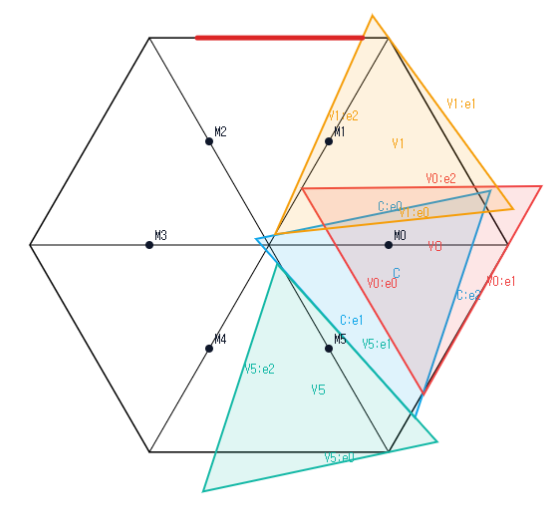
\includegraphics[width=.78\linewidth]
  {figures/strategy2_ce1_ce2_n0_all_vd0.png}
\caption{Schematic view of the common CE1/CE2, $N_+=0$, all-Vd0 boundary
package, not to scale.  The C triangle and three representative Vd0 vertex
triangles are shown; the remaining three triangles are omitted for readability.  The
simultaneous placement is not a candidate cover, and no proof depends on
visual inspection.}
\label{fig:ce1-ce2-n0-all-vd0}
\end{figure}

\begin{proposition}[Nonzero-gap all-Vd0 skeleton-data obstruction]
\label{prop:nplus-zero-all-vd0}
Let the C triangle be CE1 or CE2. Assume all six V triangles are Vd0,
\[
 A_i+B_i\le1\qquad(i=0,\ldots,5),
\]
the seven open triangles cover the full skeleton
\[
 S=\partial H\cup\bigcup_{i=0}^5r_i,
\]
and assume $N_{\mathrm{gap}}\ge1$.  Then no such configuration exists; in
particular, these data cannot cover all of $H$.
\end{proposition}

\begin{proof}
Let $d_i^C$ be the center reach on $r_i$, measured from $O$, and set
$c_i^C=1-d_i^C$. Since every V triangle is Vd0,
$\Haus(T_{i-1}\cap r_i)=\Haus(T_{i+1}\cap r_i)=0$; diameter locality
excludes every $T_j$ with $j\notin\{i-1,i,i+1\}$.
Skeleton coverage therefore forces
\[
 C_i\ge c_i^C\qquad(i=0,\ldots,5).
\tag{\(*\)}
\]

Let $N_{\mathrm{gap}}$ be the number of positive center traces containing a
boundary gap. Singleton boundary gaps are included. By hypothesis and the
center classification, $N_{\mathrm{gap}}\in\{1,2\}$, with
$N_{\mathrm{gap}}=1$ in CE1.

Suppose $N_{\mathrm{gap}}=1$. Normalize the active trace to
\[
 I_R=\left[\frac{k}{R},W+\delta\right]\subset e_{0,1}
\]
and put
\[
 s=\frac{k}{R},\qquad q=R-\delta.
\]
Gap containment gives $B_0\ge s$ and $A_1\ge q$. The companion edge is
absent or gap-free, so $A_0+B_5\ge1$; since $A_0+B_0\le1$, one has
$B_5\ge s$. By \((*)\),
\[
 C_1\ge1-\frac\delta R,
 \qquad
 C_5\ge1-\frac\alpha W.
\]
The exact one-side endpoint theorem gives
\[
 M_{1-\alpha/W}(s)
 +M_{1-\delta/R}(q)<1.
\]
The three internal V triangles $T_2,T_3,T_4$ lie on a center-free boundary
path. The path budget forces their total boundary contribution above three,
contrary to their three nonsupercritical caps.

If $N_{\mathrm{gap}}=2$, the center is CE2. The paired endpoint theorem, together
with \((*)\), gives
\[
 p=W-\alpha,\qquad q=R-\delta,
 \qquad \overline M_{p/W}(p)+\overline M_{q/R}(q)<1.
\]
The same center-free three-V triangle path gives the contradiction.

The two nonzero gap ranks are exhaustive.
\end{proof}

We next treat the additional T3-like V triangles in the $N_+=0$ branch.  The
following local facts also reappear later.

\begin{lemma}[T3-like midpoint and side tradeoff]
\label{lem:t3-midpoint-tradeoff}
Let $T_i$ be T3-like.  Then $M_i\notin T_i$.  After applying the closed-trace
domination of Proposition~\ref{prop:t3-translation}, suppose
$\Haus(T_i\cap r_{i+1})>0$ and $M_{i+1}$ belongs to the dominated trace.
If $b$ is its boundary reach toward $V_{i+1}$, $c$ its exit on $r_i$, and
$\ell$ its entry on $r_{i+1}$, all measured from the relevant
vertex, then
\begin{equation}
 b+c<1,\qquad b+\ell>1.
 \label{eq:t3-side-tradeoff}
\end{equation}
Consequently two T3-like traces $T_i,T_{i+1}$ that cover each other's
midpoint, with positive traces on $r_{i+1}$ and $r_i$, respectively, cannot
cover both segments $[V_i,M_i]$ and $[V_{i+1},M_{i+1}]$ if no other triangle
has positive trace there.
\end{lemma}

\begin{proof}
Apply Proposition~\ref{prop:t3-translation} and reflect if necessary.  Its
translated Type-II majorant has parameters
\[
 0<t<1,\qquad z=\sqrt{1-t+t^2},\qquad \alpha=0,\qquad 0<\beta<z.
\]
Its wedge vertex has
\[
 Q_x=\frac{z-t\beta}{1-t+t^2}>1.
\]
Hence
\[
 t\beta<z-z^2.
\]
The majorant's radial exit is $c=\beta/(1-t)$.  Since
\[
 (1-z)(1+z)=t(1-t),
\]
we obtain
\[
 c<\frac{z-z^2}{t(1-t)}=\frac{z}{1+z}<\frac12.
\]
Here $z<1$ because $0<t<1$.  Thus the translated majorant misses $M_0$,
and its closed-trace domination
implies that the original T3-like triangle misses $M_0$ as well.

For the tradeoff, the translated T3-like trace has the exhaustive Type-II
form
\[
 \begin{aligned}
 (1-t)x+ty&\ge0,\\
 \beta+tx-y&\ge0,\\
 \beta+x-(1-t)y&\le z,
 \end{aligned}
 \qquad 0<t<1,\quad z=\sqrt{1-t+t^2},\quad0<\beta<z.
\]
For the selected support on $r_1$, substitution in the Type-II half-planes
gives
\[
 b=z-\beta,\qquad c=\frac{\beta}{1-t},\qquad
 \ell=\frac{\beta+1-z}{1-t}.
\]
The condition $M_1\in T$ is
$\beta\le z-(1+t)/2$.  Therefore
\[
 b+c\le z+\frac{t}{1-t}
 \left(z-\frac{1+t}{2}\right)
 =1-\frac{(1-z)^2}{2(1-t)}<1,
\]
whereas
\[
 b+\ell-1=\frac{t(1-z+\beta)}{1-t}>0.
\]
For a crossed adjacent pair, write $(b,c,\ell)$ for the first triangle's
boundary reach, own-arm exit, and opposite-arm entry, and write
$(\widetilde b,\widetilde c,\widetilde\ell)$ for the reflected quantities of
the second.  Equation~\eqref{eq:t3-side-tradeoff} and its reflection give
\[
 b+c<1,\quad b+\ell>1,\qquad
 \widetilde b+\widetilde c<1,\quad
 \widetilde b+\widetilde\ell>1.
\]
Coverage forces $c\ge\widetilde\ell$ and
$\widetilde c\ge\ell$.  The first inequality gives
$\widetilde b+c>1>b+c$, hence $\widetilde b>b$; the second gives
$b+\widetilde c>1>\widetilde b+\widetilde c$, hence
$b>\widetilde b$, a contradiction.
\end{proof}

\begin{lemma}[The support-isolated four-branch inequality]
\label{lem:407-four-label-loss}
\label{thm:s2-geom-t3}
Assume the support-isolated T3-like endpoint state of
Definition~\ref{def:body-t3-endpoint-state}.  Then the two endpoint V triangles
satisfy
\begin{equation}
 \overline M_{c_5^\ast}(a_5^\ast)+\overline M_{c_1^\ast}(a_1^\ast)<1,
 \label{eq:407-loss}
\end{equation}
where $a_1^\ast,a_5^\ast$ are the exact boundary inputs and
$c_1^\ast,c_5^\ast$ the exact radial lower bounds defined there.
\end{lemma}

\begin{proof}
Use the CE1 side variables $0<\lambda<1$,
$\rho=\sqrt{1-\lambda+\lambda^2}$ and center slacks
\[
 X=F_0(O),\qquad Y=F_2(O).
\]
Then
\[
 a_C=\lambda-Y,\qquad
 \lambda s=X+Y+1-\rho,
\]
and Proposition~\ref{prop:signed-center-normal-form} gives
\[
 \rho-X-Y>\frac12,\qquad
 \frac Y\lambda<\frac12,\qquad
 \frac X{1-\lambda}<\frac12.
\]
Consequently the apparent minima in the two radial exits collapse to
\[
 \gamma_1=\frac Y\lambda,\qquad
 \gamma_5=\frac X{1-\lambda}.
\]
For CE2 the second boundary interval is $[S,T]$, where
\[
 S=\frac{X+Y+1-\rho}{1-\lambda},\qquad T=X+\lambda.
\]

The T3-like normal form supplies $D>1$, $0<R<1$, and $\alpha,p\ge0$ with
\[
 R^2-DR+D^2=1,\qquad \alpha+p=1/D,\qquad
 q=1-p=\alpha+(D-1)/D<1/2.
\]
Its interval on $r_1$, measured from $V_1$, is
\[
 [c,u],\qquad c=Dq/R,\qquad u=q+(1-R)/D.
\]
Using the residual operator \eqref{eq:reader-residual-operator}, the exact
boundary inputs are, with $J_1=[s,t]$ and with $J_5=[S,T]$ in CE2 but
$J_5=\varnothing$ in CE1,
\[
 a_1^\ast=\mathcal R_{J_1}(p),\qquad
 a_5^\ast=\mathcal R_{J_5}(\alpha),
\]
and
\[
 c_5^\ast=1-\gamma_5,\qquad
 c_1^\ast=
 \begin{cases}
 c,&1-u\le\gamma_1\le1-c,\\
 1-\gamma_1,&\text{otherwise}.
 \end{cases}
\]

If $a_1^\ast+a_5^\ast>1$, the two caps already imply
$\overline M_{c_5^\ast}(a_5^\ast)+\overline M_{c_1^\ast}(a_1^\ast)<1$.  Assume the hard region
$a_1^\ast+a_5^\ast\le1$.  The following table is an exhaustive case analysis of the four
possible first branches; the middle column states the exact decisive
inequality.
\[
\begin{array}{c|c|c}
\text{first branch}&\text{right branches}&\text{conclusion}\\ \hline
\mathrm{Const}&\mathrm{Lin}&e(\gamma_5)<a_1^\ast\\
\mathrm{Const}&\mathrm{Const},Q_-&\overline M_{c_5^\ast}(a_5^\ast)+\overline M_{c_1^\ast}(a_1^\ast)<1\\
\mathrm{Const}&Q_+&e(\gamma_5)<a_1^\ast\\
Q_-&\mathrm{Const},Q_-&\overline M_{c_5^\ast}(a_5^\ast)+\overline M_{c_1^\ast}(a_1^\ast)<1\\
Q_-&\mathrm{Lin},Q_+&\overline M_{c_5^\ast}(a_5^\ast)<a_1^\ast\\
\mathrm{Lin}&\text{all}&\text{impossible}\\
Q_+&\mathrm{Lin},Q_+&\text{impossible}\\
Q_+&\mathrm{Const},Q_-&\overline M_{c_5^\ast}(a_5^\ast)+\overline M_{c_1^\ast}(a_1^\ast)<1.
\end{array}
\]
We verify the nonformal entries.  Put
$\kappa=(1-\rho)/(1-\lambda)$.  From
$X+(1-\lambda)Y<\rho(1-\rho)$ one obtains
\begin{align}
 \gamma_1\ge a_C&\Longrightarrow e(\gamma_5)<a_C,
 \label{eq:407-core-estimate}\\
 S\le Y/\lambda&\Longrightarrow e(\gamma_5)<S.
 \label{eq:407-S-estimate}
\end{align}
For \eqref{eq:407-core-estimate}, one has
$\gamma_5<a_C-\kappa$ and
$a_C-\kappa<1/8$; then \eqref{eq:low-root-bounds} applies, and the remaining
comparison is
\[
 (a_C-\kappa)+5(a_C-\kappa)^2\le\kappa.
\]
After squaring its positive sides, the difference is
$\lambda(23\lambda^3+58\lambda^2+7\lambda+72)>0$.
For \eqref{eq:407-S-estimate}, combine the premise with the center
inequality and put $x=\lambda$.  This gives $0<x<3/8$ and
\[
 X<X_*=\frac{(1-\rho)(\rho(1-2x)-x(1-x))}{1-x-x^2}.
\]
Set
\[
 \delta=\frac{1-\rho}{1-x}=\frac{x}{1+\rho},\qquad
 \eta=\frac{X}{1-x},\qquad
 f=\rho(1-2x)-x(1-x),\qquad d=1-x-x^2.
\]
Then $\gamma_5\le\eta<\delta f/d$.  Moreover
\[
 \frac fd<1-2x,
\]
because, after multiplication by positive denominators, this is just
\[
 \rho<d+\frac{x(1-x)}{1-2x}
 =1+\frac{2x^3}{1-2x}.
\]
Hence $\eta<\delta(1-2x)<1/8$.  If $\eta=0$, the assertion is immediate.
Otherwise,
\[
 S\ge\frac{X+1-\rho}{1-2x}
 =\frac{1-x}{1-2x}(\eta+\delta)
 >2\eta\left(\frac{1-x}{1-2x}\right)^2.
\]
On the other hand,
\[
 5\eta<5\delta(1-2x)
 <2\left[\left(\frac{1-x}{1-2x}\right)^2-1\right].
\]
For the middle sign use $\rho>1-x$ and
\[
2(2-3x)(2-x)-5(1-2x)^3
 =(4x-3)(10x^2-6x-1)>0
 \qquad(0<x<3/8).
\]
Indeed both factors are negative; for the quadratic use
$10x^2\le15x/4<6x+1$.
The low-root estimate \eqref{eq:low-root-bounds} now gives
\[
 e(\gamma_5)\le2\gamma_5+5\gamma_5^2
 \le2\eta+5\eta^2<S,
\]
proving \eqref{eq:407-S-estimate} without any polynomial coefficient list.
The constant-branch separation follows from its exact polynomial: if its output is
$z=e(\eta)$ at input $1-\beta$, then
\[
 \beta\ge z+\eta.
 \label{eq:407-L-separation}
\]
Indeed the selector polynomial
$P(x,z)=x^4-4x^3+5x^2-(2+z)x+z-z^2$ is strictly decreasing on the low
range and vanishes at $x=\eta$.  Equations
\eqref{eq:407-core-estimate}--\eqref{eq:407-L-separation}, with the three
residual cases in $\mathcal R_J$, prove every first-constant entry.  For a first $Q_-$
branch the exact root test
\[
 Q_-(a,c)<z\iff c^2(a+z)^2-(a^2-ac+c^2)>0
\]
is increasing in $z$.  Substitution of $a_1^\ast$, followed by the center
inequality, proves $\overline M_{c_5^\ast}(a_5^\ast)<a_1^\ast$ except in the low--low entries, which
are immediate from $Q_-(a,c)\le\min\{a,1-a\}$ and the constant-branch output is below $1/2$.
First-coordinate linear would force either
$X\ge(1-\lambda)\alpha$ and $Y\ge\lambda-\alpha$, contradicting
$s\le p$, or, in the CE2 overlap case, $S\ge1/2$, contradicting
$S\le\alpha<1/2$.

For a first $Q_+$ branch put $r=1-\lambda$,
$y=Y/\lambda$ and choose $\beta$ so that
\[
 m=\sqrt{\beta^2-\beta+1},\quad
 1-\gamma_5=\frac m{r+\beta},\quad
 \overline M_{c_5^\ast}(a_5^\ast)=\frac{\beta m}{r+\beta}.
\]
The exact selector is
\begin{equation}
 \beta\ge\max\left\{r,\frac12,\frac{1-r^2}{1+2r}\right\},\qquad
 r\ge(1-\beta)(r+\beta)^2.
 \label{eq:407-high-domain}
\end{equation}
The center inequalities give $y<1/10$ and, with
\[
 y_*=\frac r{1-r}
 \left(\frac m{r+\beta}-\frac12-\frac{1-r}{1+\sqrt{r^2-r+1}}\right),
\]
give $y<y_*$ and
\[
 3y_*\le1-\frac{\beta m}{r+\beta}.
\]
This proves the right-constant entry by $e(y)<3y$.  It excludes right linear and
right high by the exact high-input filter.  For right $Q_-$ with input
$a_C$, direct substitution gives a sum below one.  For input $q$, put
$c=1-y$, $q=tc$, and let $\widehat b_1=\overline M_{c_1^\ast}(q)$.  The selected $Q_-$ equations
give
\[
 \widehat b_1\le\kappa:=\frac{\sqrt{13}-1}{6},\qquad
 q\le\tau<\frac{93}{200},
\]
where $\tau\in(0,1/2)$ is the unique root of
$\tau^4-3\tau^3+3\tau^2-3\tau+1=0$.  In this CE2 overlap subcase the
support ordering gives $q>S$.  The common left-high identities are
\[
 S=S_0+\frac{1-r}{r}y,\qquad
 S_0=1-\frac{m}{r+\beta}+\frac{1-r}{1+\sqrt{r^2-r+1}}.
\]
Since $y>0$, we have the complete chain
\[
 S_0<S<q\le\tau<\frac{93}{200}.
\]
We now replace the former interval subdivision by a one-variable comparison.
Write $s=r+\beta$ and $\rho_r=\sqrt{r^2-r+1}$.  The selected Cell~2
inequality factors as
\[
 r-(1-\beta)(r+\beta)^2
 =(s-1)(\beta^2+r\beta-r).
\]
The second factor is nonnegative because $r\le\beta$ and $\beta\ge1/2$;
if it vanishes, then $r=\beta=1/2$.  Hence $s\ge1$.  It follows that
$\rho_r\le m$, since
$\rho_r^2-m^2=(r-\beta)(s-1)\le0$.

Define the one-variable lower bound
\[
 \overline S(\beta)=1-m+\frac{\beta}{1+m}.
\]
Then
\[
 S_0\ge1-\frac m s+\frac{1-r}{1+m}\ge\overline S(\beta).
\]
Indeed, the second difference is
\[
 (s-1)\left(\frac m s-\frac1{1+m}\right)\ge0.
\]
For the last sign use $s\le2\beta\le m(1+m)$: if
$\gamma_\beta=3\beta-\beta^2-1$, then $\gamma_\beta>0$ and
\[
 m^2-\gamma_\beta^2=-\beta(\beta-1)(\beta^2-5\beta+5)\ge0,
 \qquad m^2+\gamma_\beta=2\beta.
\]

Put $\beta_0=5657/10000$, $T=93/200$, and $\beta_*=161/250$.
If $\beta m/s\ge\beta_0$, then $\beta m\ge\beta_0$. The function
$\phi(\beta)=\beta m$ is strictly increasing, and the exact comparison
\[
 \beta_0^2-\beta_*^2m(\beta_*)^2
 =\frac{22782769}{62500000000}>0
\]
therefore gives $\beta>\beta_*$.  On $[\beta_*,1]$ put
\[
 \chi(\beta)=\frac{107}{200}-Tm-(1-\beta)^2.
\]
Since $\chi''=-3T/(4m^3)-2<0$, the function $\chi$ is concave. Its endpoint
values are positive: $\chi(1)=7/100$, while, for
$a_*=107/200-(1-\beta_*)^2=51033/125000$,
\[
 a_*^2-T^2m(\beta_*)^2
 =\frac{1693881}{62500000000}>0.
\]
Thus $\chi>0$ throughout the interval. The identity
\[
 (\overline S(\beta)-T)(1+m)=\chi(\beta)
\]
shows that $\beta m/s\ge\beta_0$ would force $S_0>T$, a contradiction.
Consequently
\[
 \overline M_{c_5^\ast}(a_5^\ast)<\frac{5657}{10000}
 <\frac{7-\sqrt{13}}6.
\]
The final strict comparison follows by squaring
$\sqrt{13}<18029/5000$, whose squared difference is
$44841/25000000>0$.
Thus the final sum is also below one.  The table is exhaustive, proving
\eqref{eq:407-loss}.
\end{proof}

\begin{proposition}[The nonzero-gap $N_+=0$ T3-like branch]
\label{prop:nplus-zero-t3}
Assume that $T_C$ is CE1 or CE2, $N_+=0$, no V triangle is Vd1 or Vd2,
at least one V triangle is T3-like, and $N_{\mathrm{gap}}\ge1$.  Then the
seven triangles do not cover $H$.
\end{proposition}

\begin{proof}
By Proposition~\ref{prop:unique-center-midpoint}, normalize so that
$T_C\cap\{M_0,\ldots,M_5\}=\{M_0\}$, and simultaneously apply the
closed-trace domination of Proposition~\ref{prop:t3-translation} to every
T3-like triangle.  If $T_0$ were not T3-like, a maximal consecutive block of
T3-like indices among $1,\ldots,5$ would have to match its triangles bijectively
to the same block of uncovered midpoints.  Each match sends $T_i$ only to
$M_{i-1}$ or $M_{i+1}$, because a T3-like triangle misses $M_i$ and an
open role $U_i$ whose closure $T_i$ is Vd0 cannot contain $M_{i-1}$ or
$M_{i+1}$.
Its first two triangles therefore form a crossed pair
forbidden by Lemma~\ref{lem:t3-midpoint-tradeoff}.  Hence $T_0$ is T3-like;
reflect so that $\Haus(T_0\cap r_1)>0$.

There are at most two T3-like triangles. Indeed, with $N_+=0$ and no
Vd1/Vd2 triangle, their number $k$ equals $N_{\mathrm{sp}}$. If $k\ge3$,
Theorem~\ref{thm:common-skeleton-count} gives an immediate full-skeleton
contradiction.
Midpoint locality then forces $T_2,T_4,T_5$ to be Vd0.  Consequently $r_1$
has positive support only from $T_C,T_0,T_1$, and $r_5$ only from $T_C,T_5$.

Thus all hypotheses of the support-isolated state in
Definition~\ref{def:body-t3-endpoint-state} hold.  The actual forward reaches
of $T_1,T_5$ are bounded by the two safe maps in
Lemma~\ref{lem:407-four-label-loss}; an extra reach lower bound on $r_0$ or
$r_2$ for a possible T3-like $T_1$ only shrinks its feasible set.  Thus their sum is
less than one.  V triangles $T_2,T_3,T_4$ must cover more than three units of the
four intervening boundary edges, while their three nonsupercritical caps
sum to at most three.  This contradiction proves the proposition.
\end{proof}

\subsubsection{Two reusable high-radial endpoint inequalities}

\begin{lemma}[One-side endpoint loss]
\label{lem:one-side-capped-loss}
\label{thm:s2-geom-e1}
Let $0<R<1$, $S=\sqrt{1-R+R^2}$, and let $s,u,w>0$ satisfy
$s+u+w=1$ and $0<u<R$.  Put
\[
 \delta=\frac{R}{1+S},\qquad
 \gamma=u-\delta-\frac{R}{1-R}w,
\]
and assume $\gamma>0$.  Set
\[
 c_1=u/R,\qquad c_5=1-\gamma.
\]
Then
\begin{equation}
 \overline M_{c_5}(s)+\overline M_{c_1}(u)<1.
 \label{eq:one-side-loss}
\end{equation}
\end{lemma}

\begin{proof}
Put $\eta=(1-R)\delta=1-S$ and
\[
 \widehat b_5=\overline M_{c_5}(s),\qquad
 \widehat b_1=\overline M_{c_1}(u).
\]
The center identity may be written
\begin{equation}
 c_5=\frac{1-u+\eta-Rs}{1-R}.
 \label{eq:one-side-center-line}
\end{equation}
The hypotheses imply $1/2<c_1,c_5<1$: for example
$u>\delta$ gives $c_1>1/(1+S)>1/2$, and
$\gamma<u-\delta<R-\delta=RS/(1+S)<1/2$ gives $c_5>1/2$.
Thus the four high-radial branches of
the four-branch high-radial map in Proposition~\ref{prop:capped-demand-map} are exhaustive.

\smallskip\noindent
\emph{Right low branches.}
If the right branch is $Q_-$, its exact frontier equation gives
$(u+\widehat b_1)^2=1-R+R^2=S^2$, so $\widehat b_1=S-u$.  For a right constant branch write
$\widehat b_1=kc_1$, $0\le k\le1/2$, and $C=1-k+k^2=c_1^2$.  With $X_R=R+k$, the
constant-branch selector factors as
\[
 q=c_1^2(X_R-1)G_k(X_R),\qquad
 G_k(X)=CX^3+CX^2-k(1-k)X+k^2.
\]
For $X\ge k$, $G_k(X)>0$: when $k>0$,
$G_k'(X)\ge k(1+2k-k^2+3k^3)>0$ and
$G_k(k)=k^2(1+k+k^3)>0$.  Hence $q\le0$ gives $X_R\le1$.  If
$h_R=1-X_R$, then
\[
 S^2-(u+\widehat b_1)^2=h_R(1+2k^2+k(1-k)h_R)\ge0.
\]
Consequently either right low branch satisfies
\begin{equation}
 \widehat b_1\le X:=S-u.
 \label{eq:one-side-right-low}
\end{equation}

\smallskip\noindent
\emph{A left low branch against right high or linear.}
For left $Q_-$ put $z=s/c_5=1-p$ and
$h=\sqrt{1-p+p^2}$.  The component selector gives
$0\le p\le1/2$, the frontier gives $s+\widehat b_5=h$, and its selector gives
$s\le(1-p)h$.  Equation \eqref{eq:one-side-center-line} becomes
$c_5(1-Rp)=1-u+\eta$, whence
\[
 u\ge \eta+(1-h)+Rph.
\]
Put $q_0=ph$.  If $q_0>R$, then
$p(1-p)>R(1-R)$ and the preceding lower bound would give $u>R$.
Thus $q_0\le R$, and
\[
 \eta+1-h>
 \frac{R(1-R)+p(1-p)}2\ge(1-R)q_0.
\]
Substitution in the exact formula
\[
 w=\frac{(1-R)(1-u)p-\eta(1-p)}{1-Rp}
\]
now gives $w<1-h$. A right high output has the form $\omega_\beta-u$, where
$\omega_\beta=\sqrt{1-\beta+\beta^2}\le1$; for linear take
$\omega_\beta=1$. Hence
\[
 \widehat b_5+\widehat b_1=h+\omega_\beta-(s+u)
 =1+w-(1-h)-(1-\omega_\beta)<1.
\]

For a left constant branch write
\[
 c_5=h(x):=\sqrt{1-x+x^2},\qquad
 \widehat b_5=xh(x),\qquad 0\le x\le\frac12,
\]
and, along the center line,
\[
 s(x)=\frac{R-u+\eta+(1-R)(1-h(x))}{R}.
\]
If $y=s(x)/h(x)$, the exact selector factorization is
\[
 \frac{q}{h(x)^2}=(y-(1-x))P_x(y),
\]
where
\begin{align*}
 P_x(y)={}&(1-x+x^2)y^3+(1+2x-2x^2+3x^3)y^2\\
 &+(x+2x^2-x^3+3x^4)y+(x^2+x^3+x^5).
\end{align*}
Every coefficient is nonnegative on $0\le x\le1/2$, and the polynomial is
positive at every nondegenerate point.  Thus a selected constant-branch point has
$s(x)\le(1-x)h(x)$.  The two curves meet once in $(0,1/2)$: at $x=0$ the
left side is smaller, while at $x=1/2$ it is enough to use
\[
 u\le\frac{R}{1+R}\quad(\mathrm{Lin}),\qquad
 u\le\min\{RS,S/2\}\quad(Q_+).
\]
Writing $e_0=1-\sqrt3/2$, the corresponding endpoint differences are
\[
 \frac{(1-R)(R^2+2Re_0+2e_0)}{2(1+R)}>0
\]
for linear, and respectively
$[2e_0(1-R)-R^3]/2\ge0$ for $R\le1/2$ and
$(1-R)(3R+4e_0-2)/4\ge0$ for $R\ge1/2$ in the high case.
At the unique transition $x_0$, the constant frontier is the $q=0$ endpoint of
the preceding $Q_-$ branch.  Since $xh(x)$ increases, every selected left constant-branch output is no larger than that transition output.  The preceding strict
loss therefore also covers $(\mathrm{Const},Q_+)$ and $(\mathrm{Const},\mathrm{Lin})$.

\smallskip\noindent
\emph{linear and high exclusions.}
Left linear forces $s<1/2$ and $\gamma\ge s$.  Right linear or right high gives
$u\le1/2$, but
\[
 \gamma-s=2u-1-\delta+\frac{1-2R}{1-R}w<0:
\]
for $R\ge1/2$ this is immediate, while for $R<1/2$ use $w<1-u$ to bound it
by $(u-R)/(1-R)-\delta<0$.  Thus left linear cannot pair with either branch.
If the left branch is high and the right one linear, then $s<1/2$ and
$u\le R/(1+R)$, whereas $\gamma>0$ and $w>1/2-u$ force
$u>R/2+\eta>R/(1+R)$; the final inequality is equivalent to
$2(1+R)>1+S$.  This pair is also impossible.

\smallskip\noindent
\emph{A right low branch.}
Use \eqref{eq:one-side-right-low}.  If $s>X$, the cap gives
$\widehat b_5+\widehat b_1<1$.  Suppose $s\le X$ and put
\[
 c_X=X+2\delta,\qquad f(c,z)=c^4-c^2+zc-z^2.
\]
At the limiting value $u=R$, with $\kappa=\delta$, one has
\[
 X_0=\frac{1-2\kappa}{1+\kappa},\qquad
 c_0=\frac{1+2\kappa^2}{1+\kappa}.
\]
Now $c_0>\sqrt3/2$ because
$16\kappa^4+13\kappa^2-6\kappa+1>0$, and
\[
 f(c_0,X_0)=
 \frac{\kappa^2(1-2\kappa)^2
 (4\kappa^4+4\kappa^3+10\kappa^2+6\kappa+5)}{(1+\kappa)^4}>0.
\]
Along the $u$-line,
$\frac d{du}f(c_X,X)=-4c_X^3+c_X+X<0$, so the same two signs hold before
the limiting endpoint.  Therefore, for
$\ell(c)=c(1-\sqrt{4c^2-3})/2$,
\[
 \ell(c_X)<X<c_X-\ell(c_X),\qquad \ell(c_X)<1-X.
\]

Write $c=h(z)=\sqrt{1-z+z^2}$ and let $z_X$ satisfy $h(z_X)=c_X$.
The actual $c_5(s)$ corresponds to $0<z\le z_X<1/2$, and
\[
 s(z)=s_0+\frac{1-R}{R}(1-h(z)),\qquad
 s_0=\frac{R-u+\eta}{R}>0.
\]
The transition input $(1-z)h(z)$ decreases, and the preceding root ordering
gives $s(z_X)<(1-z_X)h(z_X)$, hence the same strict inequality for all
$z\le z_X$.  To check the order of the two boundary coordinates put
\[
 \phi(z)=s(z)-zh(z),\qquad k_R=\frac{1-R}{R}.
\]
Its endpoint values are $s_0>0$ and $X-\ell(c_X)>0$.  Moreover
\[
 \phi'(z)=\frac{(k_R+z)(1-2z)}{2h(z)}-h(z).
\]
For $k_R\le2$ this is nonpositive; for $k_R>2$ its zero is described by the
strictly increasing function
$K_0(z)=(2-3z+4z^2)/(1-2z)$, so the minimum is again at an endpoint.
Thus $zh(z)<s(z)$.  Applying the already displayed polynomial $P_z$ gives
the strict constant-branch selector, and
$s+zh(z)\le X+\ell(c_X)<1$.  Since
$\partial_bF_L=c(1-2z)>0$ and each feasible fiber is an interval, the nonsupercritical
maximum is
\[
 \widehat b_5\le zh(z)\le z_Xh(z_X)=\ell(c_X)<1-X.
\]
Together with $\widehat b_1\le X$, this proves the loss for every right low branch.

\smallskip\noindent
\emph{High--high.}
Let $c_L(z)$ be the unique root in $[\sqrt3/2,1]$ of $f(c,z)=0$.
With $D_c=4c^3-2c+z>0$, implicit differentiation gives
\[
 c_L''(z)=
 \frac{2(c^2-cz+z^2)+16c^2z(c-z)}{D_c^3}>0.
\]
A selected left high branch requires $s<1/2$ and $c_5(s)\le c_L(s)$.
Define
\[
 s_0=\frac{R-u+\eta}{R};
\]
then $0<s_0<s$ and $c_5(s_0)=1$.  The explicitly named function
$\psi_L(z)=c_5(z)-c_L(z)$ is concave, with $\psi_L(s_0)>0$.  The right high bound
$u\le\min\{RS,S/2\}$ gives $c_5(1/2)>7/8$.  For $R\le1/2$ this follows
after squaring from
$17-10R+9R^2-64R^3-64R^4>0$ (a decreasing polynomial with value $9/4$ at
$1/2$); for $R\ge1/2$ it follows from
$(3+R)^2-16S^2=(1-R)(15R-7)>0$.  Finally
\[
 f(7/8,1/2)=33/4096>0
\]
and $f$ increases in $c$ on this range, so $c_L(1/2)<7/8$ and
$\psi_L(1/2)>0$.  Concavity contradicts $\psi_L(s)\le0$.  Thus high--high is
impossible.

If both branches are low, the cap already gives
$\widehat b_5+\widehat b_1\le s+u=1-w<1$.  The preceding five paragraphs cover every other
ordered pair of the four branches, proving \eqref{eq:one-side-loss}.
\end{proof}

\begin{lemma}[CE2 two-endpoint loss]
\label{lem:two-endpoint-capped-loss}
\label{thm:s2-geom-e2}
Let $[x,U]$ and $[y,v]$ be the two exact CE2 traces in the legacy
coordinates of Remark~\ref{rem:signed-legacy-variables}, where $U$ denotes
the endpoint called $u$ there.  Put
\[
 p=1-U,\qquad q=1-v,\qquad
 r=\frac{x}{x+y},\qquad w=\frac{y}{x+y},
\]
and reflect if necessary so that $0<w\le1/2$ and $r=1-w$.  Then
\begin{equation}
 \overline M_{p/w}(p)+\overline M_{q/r}(q)<1.
 \label{eq:two-endpoint-loss}
\end{equation}
\end{lemma}

\begin{proof}
Put
\[
 S_0=x+y,\quad K=\sqrt{1-wr},\quad
 z=\frac{w}{1+K},\quad\zeta=\frac{r}{1+K},
 \quad\alpha=\frac pw,\quad\beta=\frac qr.
\]
Then $D=S_0K$, $1-K=wr/(1+K)$, and the exact midpoint inequalities give
$1/2<\alpha,\beta<1$.  Dividing the coupling equation
$(U+v)S_0-xy=D$ by $S_0$, and using successively $x<U$ and $y<v$, gives
the strict endpoint inequalities
\begin{equation}
 \beta+p>1+z,\qquad \alpha+q>1+\zeta.
 \label{eq:ce2-strict-endpoints}
\end{equation}
Define the local outgoing-cap functions
\[
 K_w(\alpha)=\overline M_\alpha(w\alpha),\qquad
 K_r(\beta)=\overline M_\beta(r\beta),\qquad
 h(t)=\sqrt{1-t+t^2}.
\]
Thus the desired sum is $K_w(\alpha)+K_r(\beta)$.

\smallskip\noindent
\emph{Selected branch parametrizations.}
For a side of weight $\sigma\in\{w,r\}$, every constant branch has
\begin{equation}
 c=h(k),\qquad \overline M_c(\sigma c)=kh(k),\qquad0\le k\le w,
 \label{eq:two-endpoint-L-param}
\end{equation}
on either side.  On the large side the range follows from
\[
 Q_{\rm cell}/h(k)^2=(k-w)G_k(r+k),
\]
where
$G_k(X)=h(k)^2X^3+h(k)^2X^2-k(1-k)X+k^2>0$ for $X\ge k$.
The remaining selected parametrizations are
\begin{align}
 \alpha&=\frac{h(a)}{w+a},&
 K_w(\alpha)&=a\alpha,& r\le a<1,
 \label{eq:two-endpoint-small-high}\\
 \beta&=\frac{h(b)}{r+b},&
 K_r(\beta)&=b\beta,& r\le b<1,
 \label{eq:two-endpoint-large-high}\\
 \beta&=\frac K{r+t},&
 K_r(\beta)&=t\beta=K-r\beta,& w\le t\le r.
 \label{eq:two-endpoint-large-tminus}
\end{align}
For example, the small-high selector factors as
\[
 h(a)^2a\left(\frac{w}{(w+a)^2}-(1-a)\right),\qquad
 w-(1-a)(w+a)^2=(a-r)(a^2+wa-w),
\]
which gives $a\ge r$; the other two factorizations are
$(b-w)(b^2+rb-r)$ and $(t-w)(r^2-wt)$, respectively.  These formulas
specify the selected geometric components, not discarded algebraic roots.

The small-side $Q_-$ branch is absent for $w<1/2$.  Large-side linear is
incompatible with the first inequality in
\eqref{eq:ce2-strict-endpoints}.  Small-side linear can pair only with the constant branch:
either high or $Q_-$ on the large side has $\beta\le K$, which would force
$p>(1+r)z>w/(1+w)$, contrary to linear.  Thus, up to the symmetric
$w=r=1/2$ tie, the exact list is
\begin{equation}
 \begin{gathered}
 (\mathrm{Lin},\mathrm{Const}),\ (Q_+,\mathrm{Const}),\
 (\mathrm{Const},\mathrm{Const}),\ (\mathrm{Const},Q_-),\\
 (\mathrm{Const},Q_+),\ (Q_+,Q_-),\ (Q_+,Q_+).
 \end{gathered}
 \label{eq:two-endpoint-pairs}
\end{equation}

Low--low sums are at most $K<1$: a constant-branch output is at most $wK$, while
\eqref{eq:two-endpoint-large-tminus} is at most $rK$.  For linear--constant, put
\[
 b_{\rm thr}=1+z-\frac{w}{1+w},\qquad
 \kappa=\frac{w}{1+(1+w)z}.
\]
linear and \eqref{eq:ce2-strict-endpoints} give $\beta>b_{\rm thr}$ and
$(1+\kappa)b_{\rm thr}=1+z$.  Direct reduction yields
\[
 b_{\rm thr}^2-h(\kappa)^2
 =\frac{w^2(A(w)+KC(w))}{D_0(w,K)}>0,
\]
where
\begin{align*}
 A(w)&=8-5w+22w^2+6w^3+5w^4+5w^5-w^6,\\
 C(w)&=8-w+14w^2+4w^3-2w^4+w^5,\\
 D_0(w,K)&=((1+w)(1+K))^2(1+K+w+w^2)^2.
\end{align*}
Both numerator polynomials are positive on $[0,1/2]$.  Since $h$ decreases
and $(1+k)h(k)$ increases there,
$\beta=h(k)>b_{\rm thr}>h(\kappa)$ implies
$(1+k)\beta<1+z$; combined with \eqref{eq:ce2-strict-endpoints}, this gives
$k\beta<p$ and hence the strict linear--constant loss.

It remains to verify the four pairs containing a high branch on the small
side.

\smallskip\noindent
\emph{$(\mathrm{Const},Q_+)$.}
Use parameters $0\le k\le w$ and $r\le t<1$:
\[
 \alpha=h(k),\quad K_w=kh(k),\qquad
 \beta=\frac{h(t)}{r+t},\quad K_r=\frac{th(t)}{r+t}.
\]
The first output and the last output increase in their parameters, while
$h(t)/(r+t)$ decreases.  If $w\le2/5$, then
\[
 K_w+K_r<wK+\frac1{2-w}<1;
\]
after using $K\le1-wr/2$, the positive cleared gap is
$P(w)=w^4-3w^3+4w^2-6w+2$, which decreases on $[0,2/5]$ and has
$P(2/5)=46/625$.  If $w\ge2/5$, the first endpoint inequality gives
$\beta>r+z\ge3/4$.  Since
$h(3/4)/(r+3/4)=\sqrt{13}/(7-4w)<3/4$, monotonicity forces $t<3/4$.
Therefore
\[
 K_w+K_r<\frac{\sqrt3}{4}+\frac{3\sqrt{13}}{20}<1.
\]

\smallskip\noindent
\emph{$(Q_+,Q_-)$.}
Use $a,t$ from \eqref{eq:two-endpoint-small-high} and
\eqref{eq:two-endpoint-large-tminus}.  Both reach lower bounds are at most $K$.
The first endpoint inequality gives
\[
 \alpha>\frac{1+z-K}{w}=\frac{1+r}{1+K}=:a_0.
\]
Thus $K>1-w^2$, which forces $w>1/3$, and comparison at $a=2/3$ forces
$a<2/3$.  The function
\[
 G(a)=\frac{(1+a)h(a)}{w+a}
\]
decreases on $[r,2/3]$, because its derivative numerator
$2a^3+(4w-1)a^2+(1-w)a+w-2$ is at most its value
$-7/54$ at $(2/3,1/2)$.  Hence $G(a)\le(1+r)K$.
Using the second endpoint inequality and
$K_r=K-r\beta$ gives
\[
 K_w+K_r<(2+r)K-1-\zeta<1.
\]
After multiplication by $1+K$, the last nonempty gap is
$r(3w-w^2-K)$; its squared comparison is
\[
 (3w-w^2)^2-K^2=w^4-6w^3+8w^2+w-1>0
\]
for $w>1/3$ (value $1/81$ at $1/3$, positive derivative thereafter).

\smallskip\noindent
\emph{$(Q_+,Q_+)$.}
Use parameters $a,b$ from \eqref{eq:two-endpoint-small-high}--
\eqref{eq:two-endpoint-large-high}.  The endpoint inequalities first force
$w>2/5$: for $w\le2/5$, the asserted contrary inequality
$K(w+1/(2r))\le1+z$ reduces, after multiplication by $2r(1+K)$, to
\[
 K(2w^2-4w+1)+2w^4-4w^3+w^2-w+1>0,
\]
which is immediate according as the coefficient of $K$ is nonnegative or,
using $K\le1$, from the decreasing polynomial
$2w^4-4w^3+3w^2-5w+2\ge172/625$.

For the auxiliary function $\mathcal G_c(t)=(1+t)h(t)/(c+t)$, the derivative numerator
$2t^3+(4c-1)t^2+(1-c)t+c-2$ is increasing on the present rectangle, so
$\mathcal G_c$ has at most one interior minimum. Endpoint comparison gives
\[
 K_w+\alpha\le\frac2{1+w},\qquad
 K_r+\beta\le\frac2{1+r}.
\]
The nontrivial endpoint signs are exactly
\[
 4-(1+r)^2(1+w)^2K^2
 =-w^2(w-1)^2(w^2-w-3)>0
\]
and
\[
 16r^2-(1+r)^4h(r)^2
 =(1-r)(r^5+4r^4+7r^3+9r^2-4r-1)>0;
\]
the bracket is increasing on $[1/2,1]$ and equals $13/32$ at $1/2$.
Weighting the two strict endpoint inequalities by $w/K^2$ and $r/K^2$
gives
\[
 \alpha+\beta>\frac{2K+1}{K(1+K)}.
\]
Consequently
\[
 K_w+K_r<\frac2{1+w}+\frac2{1+r}
 -\frac{2K+1}{K(1+K)}<1.
\]
The numerator of the last gap is $3Kwr-Q(w)$, where
$Q(w)=w^4-2w^3+7w^2-6w+2>0$.  Its squared difference is
\[
 D(w)=-w^8+4w^7-9w^6+13w^5-41w^4+65w^3-55w^2+24w-4.
\]
Here $D'(w)=(1-2w)P_*(w)$ with
\[
 P_*(w)=4w^6-12w^5+21w^4-22w^3+71w^2-62w+24>0
\]
on $[2/5,1/2]$; use
$71w^2-62w+24\ge743/71$ and the remaining cubic block at least $-11/4$.
Thus $D$ increases and $D(2/5)=4904/390625>0$, proving the claim.

\smallskip\noindent
\emph{$(Q_+,\mathrm{Const})$.}
Use the fully specified parameters
\[
 \alpha=\frac{h(t)}{w+t},\quad p=w\alpha,\quad b=t\alpha,
 \quad\frac12\le t<1,
\]
and
\[
 \beta=\rho=h(k),\quad \widehat b_L=k\rho,\quad 0\le k\le w.
\]
Since $p+b=h(t)$, the first endpoint inequality gives
\begin{equation}
 1-(b+k\rho)>G:=2+z-h(t)-(1+k)\rho.
 \label{eq:two-endpoint-high-L-G}
\end{equation}
Put
\[
 p_0=1+z-K=\frac{w(2-w)}{1+K},
\]
let $t_0\in(1/2,1)$ be the unique point with
$p(t_0)=wh(t_0)/(w+t_0)=p_0$, and put $b_0=t_0p_0/w$.
The exact endpoint lemma is
\begin{equation}
 b_0<1-wK.
 \label{eq:two-endpoint-b0}
\end{equation}
To verify it, set $b_*=1-wK$ and $T_*=wb_*/p_0$.  One has $0<T_*<1$, and
\[
 p_0^2(w+T_*)^2-w^2h(T_*)^2
 =-\frac{w^3(KE(w)+J(w))}{(1+K)^2(2-w)^2}>0,
\]
where
\[
 E(w)=2w^5+3w^3-20w^2+23w-6,
\]
\[
 J(w)=w^6+8w^5-22w^4+12w^3+6w^2+2w-6.
\]
Here $J\le-111/64$; if $E>0$, then
$KE+J<E+J<0$, because $E+J$ is increasing and equals $-139/64$ at
$w=1/2$.  Thus $p(T_*)<p(t_0)$.  Since $p(t)$ decreases,
$t_0<T_*$ and \eqref{eq:two-endpoint-b0} follows.

Finally put $P=1+z-p$.  If $P<K$, then $t<t_0$ and $k\le w$, so
\[
 G>2+z-h(t_0)-(1+w)K=1-b_0-wK>0.
\]
If $P\ge K$, then $K\le P\le P_1:=1+z-w/(1+w)\le1$ and there is
$a\in[0,w]$ with $h(a)=P$. Since $P<\rho$, one has $k<a$ and
$(1+k)\rho<(1+a)P=P+\ell(P)$, where
$\ell(P)=P(1-\sqrt{4P^2-3})/2$.  Hence
\[
 G>\mathcal D(P):=1-b(P)-\ell(P).
\]
This function is concave.  Indeed $\ell''(P)>0$, and the high output $b$ is
convex in $p=1+z-P$: with
$A_t=2+w-(1+2w)t>0$ and
$Q_t=8wt^2+4t^2-8wt-13t-w+4<0$,
\[
 \frac{d^2b}{dp^2}=-\frac{2h(t)(t+w)^3Q_t}{w^2A_t^3}>0.
\]
At $P=K$, \eqref{eq:two-endpoint-b0} gives
$\mathcal D(K)=1-b_0-wK>0$.  At $P=P_1$, set
$\kappa=w/(1+(1+w)z)$.  The linear--constant comparison already proved gives
$P_1>h(\kappa)$, hence
$\ell(P_1)<\kappa P_1=w/(1+w)$, while $b(P_1)=1/(1+w)$.
Thus $\mathcal D(P_1)>0$, and concavity gives $G>0$ throughout.
Equation \eqref{eq:two-endpoint-high-L-G} proves the final hard pair.

The exact list \eqref{eq:two-endpoint-pairs} is now exhausted, proving
\eqref{eq:two-endpoint-loss}.
\end{proof}

\subsubsection{The exactly-one-Vd1/Vd2 placements}

We now assume CE2, $N_+=1$, and exactly one V triangle is Vd1 or Vd2.  The corner
normal form of Proposition~\ref{prop:vd-corner-normal-form} will be used in
the following form: for some $t>0$ and $d=\sqrt{t^2+t+1}$,
\begin{equation}
 x-(t+1)y\le a,\qquad ty-(t+1)x\le tb,\qquad
 tx+y\le d-a-tb.
 \label{eq:vd-corner-form}
\end{equation}
In particular $a+b<1/2$ for the Vd1/Vd2 triangle in this corner normal
form.

\begin{lemma}[Vd1 adjacent rescue]
\label{lem:vd1-adjacent-rescue}
Assume an original open-triangle skeleton cover in the CE2 branch with
$T_C\cap\{M_0,\ldots,M_5\}=\{M_0\}$,
with $T_0$ the unique Vd1 V triangle, $M_1\in T_0$, $T_1$ uniquely supercritical,
$T_2,\ldots,T_5$ nonsupercritical Vd0, and
\[
 \Haus(T_i\cap r_{i-1})=\Haus(T_i\cap r_{i+1})=0
 \qquad(i=1,\ldots,5).
\]
Then the perimeter together with $r_1$ is not covered.
\end{lemma}

\begin{proof}
Lemma~\ref{lem:short-vd1-rescuer-profile} proves the two local inequalities
in \eqref{eq:signed-rescuer-local}.  Midpoint and support isolation force the
center to cover the $O$-side radial gap before the Vd1 interval.  The result is
therefore Corollary~\ref{cor:signed-adjacent-rescuers}.
\end{proof}

\begin{lemma}[Vd1-pair replacement interface]
\label{lem:vd1-pair-replacement}
In the remaining adjacent Vd1--supercritical placement, the pair can be
replaced by two open nonsupercritical Vd0 triangles while preserving full skeleton
coverage.
\end{lemma}

\begin{proof}
This is Proposition~\ref{prop:paper-vd1-pair-replacement}, which uses separate
local charts at the two distinguished vertices and proves all reach, triangle, and
skeleton-preservation claims explicitly.
\end{proof}

\subsubsection{Final boundary-propagation cases}

\begin{proposition}[Cases excluded by local reach certification]
\label{prop:demand-branches}
Finite-enclosure reach certification proves the following nonzero-gap exclusions; in
every item $N_{\mathrm{gap}}\ge1$:
\begin{enumerate}
\item CE1 or CE2, $N_+=0$, all V triangles Vd0;
\item CE1 or CE2, $N_+=0$, with at least one T3-like triangle and no Vd1/Vd2;
\item CE1 or CE2, $N_+=1$, all V triangles Vd0;
\item CE1 or CE2, $N_+=1$, exactly one T3-like triangle and no Vd1/Vd2;
\item the CE2, $N_+=1$, exactly-one-Vd1/Vd2 branch with no T3-like
triangle.
\end{enumerate}
All gap alternatives include singleton gaps.
\end{proposition}

\begin{proof}
The first four items are respectively Propositions
\ref{prop:nplus-zero-all-vd0}, \ref{prop:nplus-zero-t3},
\ref{prop:nplus-one-all-vd0}, and \ref{prop:nplus-one-one-t3}.
For item~5, Table~\ref{tab:ce2-one-vd-placement-cases} separates the
propagation placements from the Method~1 complements.  The propagation
placements are Lemmas \ref{lem:signed-vd-adjacent-placement} and
\ref{lem:signed-vd-nonadjacent-placement},
Corollary~\ref{cor:signed-adjacent-rescuers}, and the replacement in
Proposition~\ref{prop:paper-vd1-pair-replacement}, whose post-replacement gap
router uses Proposition~\ref{prop:length-branches} at zero gap and
Proposition~\ref{prop:nplus-zero-all-vd0} at nonzero gap rank.  The common skeleton count and
Proposition~\ref{prop:ce2-vd2-midpoint-length} close the two Method~1
complements, and Proposition~\ref{prop:paper-ce2-one-vd-placements} assembles
the partition.  The strictness at open handoffs appears in
the weak endpoint bounds, the nonattained supercritical envelope, and the
strict replacement margins; no positive-length assumption is made about a
boundary gap itself.
\end{proof}

% ---- Complete 407X case analysis and two-chart replacement ----

\subsection{The Vd1--supercritical replacement}
\label{sec:strategy2-rigor-completion}

The complete four-branch T3 endpoint calculation is already
Lemma~\ref{lem:407-four-label-loss}; its authenticated source crosswalk is
kept in the paper source ledger rather than printed a second time.  What
remains here is the unique two-chart replacement needed for the Vd branch.

\begin{proposition}[Vd1--supercritical two-chart replacement]
\label{prop:paper-vd1-pair-replacement}
Assume the CE2 branch with $N_{\mathrm{gap}}\in\{1,2\}$ in which an adjacent
Vd1 triangle and the unique supercritical Vd0 triangle lie away from the V
triangle at the center's unique midpoint.  After reflection, write their base
vertices as $V_\tau,V_{\tau+1}$.
Assume the shared boundary edge is center-free, all other V triangles are
nonsupercritical Vd0, and
\[
 \Haus(T_j\cap r_\tau)=\Haus(T_j\cap r_{\tau+1})=0
 \qquad(j\notin\{\tau,\tau+1\}).
\]
Then the pair can be replaced by two open
nonsupercritical Vd0 triangles while preserving coverage of the full skeleton.
Let $N'_{\mathrm{gap}}$ count the positive C-triangle boundary traces that
contain a gap in the replacement V traces.  If $N'_{\mathrm{gap}}=0$, the
replacement is closed by Method~1; if $N'_{\mathrm{gap}}\ge1$, it is closed
by Method~2.  No equality between $N'_{\mathrm{gap}}$ and the original
$N_{\mathrm{gap}}$ is asserted.
\end{proposition}

\begin{proof}
After a fresh cyclic renumbering, let the Vd1 triangle be based at $V_0$, the
supercritical triangle at $V_1$, and let the Vd1 triangle contain $M_1$. Write $a,b$
for the Vd1 boundary reaches and use the Vd corner parameter $t\ge1$, with
$d=\sqrt{t^2+t+1}$. Put
\[
 c=\frac{d-a-tb}{t+1},\qquad
 \lambda=\frac{t(1-b)}{t+1},\qquad
 u_{\rm adj}=\frac{d-a-tb-1}{t}.
\]
The strict midpoint and one-sided-support inequalities give
\[
 a+c<1,\qquad a<\lambda\le\frac12,
 \qquad b<\frac12,
 \qquad u_{\rm adj}<1-a.
\tag{1}
\]

Let $(A_1,B_1,C_1)$ be the maximal reaches of the supercritical triangle. The
center-free shared edge and radial coverage give
\[
 A_1\ge1-b>\frac12,
 \qquad C_1\ge\lambda.
\]
The selected supercritical admissible cell has $C_1\le1/2$. The half-square
lemma
\[
 (x,y,z)\in\mathcal A,\qquad x\ge\frac12,\qquad z\le\frac12
 \quad\Longrightarrow\quad y\le1-z
\]
therefore gives $B_1\le1-C_1\le1-\lambda$, and hence
\[
 a+B_1<1.
\tag{2}
\]
If $c_1^{\rm req}=1-d_1^C$ is the vertex-side beginning of the center trace
on $r_1$, open skeleton coverage gives
\[
 c_1^{\rm req}<\max\{C_1,u_{\rm adj}\}
 \le\max\{1-B_1,1-a\}.
\tag{3}
\]

Choose $p_2\in(a,1-B_1)$ with
\[
 \max\{p_2,1-p_2\}>c_1^{\rm req};
\]
such a point exists because the supremum of the left side on that interval is
$\max\{1-B_1,1-a\}$. Then choose
\[
 a<p_1<p_2,
 \qquad p_1<\frac12,
 \qquad1-p_1>c.
\]
Finally choose $\varepsilon>0$ smaller than
\[
 p_1-a,\quad p_2-p_1,\quad1-B_1-p_2,\quad1-p_1-c,
 \quad\max\{p_2,1-p_2\}-c_1^{\rm req}.
\tag{4}
\]

Use two distinct local charts:
\[
 X_0(x,y)=V_0+x(V_5-V_0)+y(V_1-V_0),
\]
\[
 X_1(x,y)=V_1+x(V_0-V_1)+y(V_2-V_1).
\]
For $p\le1/2$ put
\[
 \Delta_p^-=\conv\{(0,1-p),(1,1-p),(0,-p)\},
\]
and for $p>1/2$ put
\[
 \Delta_p^+=\conv\{(p,0),(p,1),(p-1,0)\}.
\]
Define
\[
 U_0'=X_0\!\left(\interior(\Delta_{p_1}^-)+(-\varepsilon,0)\right)
\]
and
\[
 U_1'=\begin{cases}
 X_1\!\left(\interior(\Delta_{p_2}^-)+(-\varepsilon,0)\right),
   &p_2\le1/2,\\
 X_1\!\left(\interior(\Delta_{p_2}^+)+(0,-\varepsilon)\right),
   &p_2>1/2.
 \end{cases}
\]

In its own chart the shifted minus template contains the origin and has reach
triple
\[
 (p-\varepsilon,1-p,1-p),
\]
while the shifted plus template contains the origin and has reach triple
\[
 (p,1-p-\varepsilon,p).
\]
In the $V_i$ chart, $i=0,1$, each closure stays strictly below the two
supporting lines of $r_{i-1}$ and $r_{i+1}$; hence
\[
 \Haus(\overline{U_i'}\cap r_{i-1})
 =\Haus(\overline{U_i'}\cap r_{i+1})=0.
\]
Thus $V_0\in U_0'$, $V_1\in U_1'$, both triangles are Vd0, and both boundary
sums equal $1-\varepsilon<1$.

The first replacement reaches beyond $a$ on $e_{5,0}$ and beyond $c$ on
$r_0$. On the shared edge its reach is $1-p_1$, while the second replacement
reaches at least $p_2-\varepsilon$ from $V_1$; their sum exceeds one by (4).
The second replacement reaches beyond $B_1$ on $e_{1,2}$ and has radial
reach $\max\{p_2,1-p_2\}>c_1^{\rm req}$ on $r_1$. Hence every boundary and
radial component formerly supplied by the special pair remains covered, and
all other skeleton components are unchanged.

The modified triangles therefore cover the full skeleton and have six
nonsupercritical Vd0 V triangles.  Let $N'_{\mathrm{gap}}$ count the positive
C-triangle boundary traces containing a gap in the modified V traces.  Since
the unchanged C triangle is CE2,
\[
 N'_{\mathrm{gap}}\in\{0,1,2\}.
\]
If $N'_{\mathrm{gap}}=0$, the zero-gap, $N_+=0$ row of
Proposition~\ref{prop:length-branches} gives the Method~1 contradiction.  If
$N'_{\mathrm{gap}}\in\{1,2\}$,
Proposition~\ref{prop:nplus-zero-all-vd0} gives the Method~2 contradiction.
These alternatives are exhaustive.  The construction does not claim that
the replacement preserves the original gap count.
\end{proof}

% ---- CE2 exactly-one-Vd placement assembly ----

\subsection{Authoritative CE2 One-Vd Placement Assembly}
\label{sec:strategy2-placement-assembly}

The following proposition is the sole CE2 exactly-one-Vd placement
assembly used by the final proof.  It cites only complete placement lemmas and
the explicit two-chart replacement in
Subsection~\ref{sec:strategy2-rigor-completion}.

\begin{proposition}[Complete CE2 exactly-one-Vd1/Vd2 assembly]
\label{prop:paper-ce2-one-vd-placements}
Assume the center has type CE2, $N_+=1$, exactly one V triangle has type Vd1
or Vd2, no T3-like triangle is present, and
$N_{\mathrm{gap}}\in\{1,2\}$.  Then the seven triangles do not cover $H$.
\end{proposition}

\begin{proof}
By Proposition~\ref{prop:unique-center-midpoint}, normalize so that
$T_C\cap\{M_0,\ldots,M_5\}=\{M_0\}$.  Let $T_\sigma$ be the unique
supercritical V triangle and let $T_\tau$ be the unique Vd1/Vd2 V triangle.
They are distinct because a Vd1/Vd2 V triangle is nonsupercritical.  The
complete nonzero-gap partition is displayed in
Table~\ref{tab:ce2-one-vd-placement-cases}; throughout that table the standing
hypothesis is $N_{\mathrm{gap}}\in\{1,2\}$.

\begin{table}[H]
\centering
\scriptsize
\renewcommand{\arraystretch}{1.08}
\begin{tabular}{p{.27\textwidth}p{.39\textwidth}p{.23\textwidth}}
\toprule
placement&chain or deficit&closing result\\
\midrule
an additional V triangle has positive support
 &upstream $N_++N_{\mathrm{sp}}\ge3$ skeleton deficit; Method~1
 &Theorem~\ref{thm:common-skeleton-count}\\
$\sigma=0$, $\tau\in\{1,5\}$
 &exact residuals, backward $\mathrm I^4$, and radial-bridge exclusion;
 the finite-enclosure reach certificate
 &Lemma~\ref{lem:signed-vd-adjacent-placement}\\
$\sigma=0$, $\tau\in\{2,3,4\}$
 &identity propagation and Vd-specific radial separation; the finite-enclosure reach certificate
 &Lemma~\ref{lem:signed-vd-nonadjacent-placement}\\
$\tau=0$ and $T_\tau$ is Vd1
 &$1-M_c^{\rm sup}$, an ordinary center-free path, and the free-envelope
 comparison; the finite-enclosure reach certificate
 &Corollary~\ref{cor:signed-adjacent-rescuers}\\
$\tau=0$ and $T_\tau$ is Vd2
 &neighboring-midpoint perimeter deficit; Method~1
 &Proposition~\ref{prop:ce2-vd2-midpoint-length}\\
$\sigma\ne0$, $\tau\ne0$, and $T_\tau$ is Vd1
 &two-chart replacement, followed by the $N'_{\mathrm{gap}}=0$ Method~1
 route or the $N'_{\mathrm{gap}}\ge1$ the finite-enclosure reach certificate route
 &Propositions \ref{prop:paper-vd1-pair-replacement},
 \ref{prop:length-branches}, and \ref{prop:nplus-zero-all-vd0}\\
$\sigma\ne0$, $\tau\ne0$, and $T_\tau$ is Vd2
 &neighboring-midpoint perimeter deficit; Method~1
 &Proposition~\ref{prop:ce2-vd2-midpoint-length}\\
\bottomrule
\end{tabular}
\caption{The complete nonzero-gap CE2 one-Vd placement partition, under the
standing hypothesis $N_{\mathrm{gap}}\in\{1,2\}$.  The first line is the
upstream pruning step before the reduced no-additional-support placement
analysis; the remaining lines are pairwise disjoint.}
\label{tab:ce2-one-vd-placement-cases}
\end{table}

For the upstream line, if an additional V triangle $T_i$ has some
$j\in\{i-1,i+1\}$ with $\Haus(T_i\cap r_j)>0$, then $T_\sigma$,
$T_\tau$, and $T_i$ give $N_++N_{\mathrm{sp}}\ge3$.  Theorem
\ref{thm:common-skeleton-count} gives the contradiction.  Hence assume the
no-additional-positive-support complement.  Every V triangle other than
$T_\sigma$ and $T_\tau$ is then nonsupercritical Vd0.

\begin{enumerate}
\item Suppose $\sigma=0$.  Since $\tau\ne0$, either
$\tau\in\{1,5\}$ or $\tau\in\{2,3,4\}$.  In the adjacent case,
Lemma~\ref{lem:signed-vd-adjacent-placement} treats both possible radial
bridges and the reflected placement.  In the nonadjacent case,
Lemma~\ref{lem:signed-vd-nonadjacent-placement} gives the strict radial
separation.

\item Suppose $\tau=0$.  The Vd1/Vd2 V triangle must rescue the midpoint
missed by $T_\sigma$, so midpoint locality gives
$\sigma\in\{1,5\}$.  If $T_\tau$ is Vd2, the neighboring-midpoint cap and
the center and supercritical perimeter caps give
Proposition~\ref{prop:ce2-vd2-midpoint-length}.  If $T_\tau$ is Vd1, the
exact Vd1 local profile and the common center-hiding theorem give
Corollary~\ref{cor:signed-adjacent-rescuers}.

\item Suppose $\sigma\ne0$ and $\tau\ne0$.  The center and $T_\sigma$
both miss $M_\sigma$, while every V triangle other than $T_\tau$ is Vd0.
Thus $T_\tau$ contains $M_\sigma$, and diameter locality makes $T_\tau$
adjacent to $T_\sigma$.  If $T_\tau$ is Vd2,
Proposition~\ref{prop:ce2-vd2-midpoint-length} applies.  If $T_\tau$ is
Vd1, the shared edge is center-free and the no-additional-support hypotheses
are exactly those of Proposition~\ref{prop:paper-vd1-pair-replacement}.
That proposition replaces the pair by two open nonsupercritical Vd0
triangles, recomputes the resulting $N'_{\mathrm{gap}}$, and routes its
zero-gap outcome to Proposition~\ref{prop:length-branches} and its nonzero-gap
outcome to Proposition~\ref{prop:nplus-zero-all-vd0}.  It makes no claim that
the replacement preserves the original gap count.
\end{enumerate}

These alternatives exhaust the relative positions of the center-midpoint V triangle,
the unique supercritical V triangle, and the unique Vd1/Vd2 V triangle.
\end{proof}


